\documentclass{article}
\usepackage[utf8]{inputenc}
\usepackage[maxcitenames=1,style=numeric, sorting = none]{biblatex}
\usepackage{amsmath}
\usepackage{amssymb}
\usepackage{amsthm}
\usepackage{tcolorbox}
\usepackage{graphicx}
\usepackage{algorithm}
\usepackage{algorithmic}
\usepackage{hyperref}
\usepackage{cleveref}
\usepackage{thmtools}
\usepackage{thm-restate}
\usepackage{enumerate}
\usepackage{xcolor}
\usepackage{textgreek}
\usepackage{caption}
\usepackage{subcaption}
\usepackage{authblk}
\usepackage{soul}
\usepackage{bm}

% \usepackage[table,xcdraw]{xcolor}
% \usepackage{subfloat}

\topmargin -.5in
\textheight 9in
\oddsidemargin -.25in
\evensidemargin -.25in
\textwidth 7in


\newcommand{\cheng}[1]{\textcolor{purple}{{\bf Cheng:~}#1}}
\newcommand{\mengyan}[1]{\textcolor{magenta}{#1}}
\newcommand{\maciej}[1]{\textcolor{blue}{#1}}

% \captionsetup[subfigure]{position=top, labelfont=bf,textfont=normalfont,singlelinecheck=off,justification=raggedright}
\captionsetup[subfigure]{font={bf,small}, skip=1pt, singlelinecheck=false}
\renewcommand{\thesubfigure}{\Alph{subfigure}}

\addbibresource{ref.bib}

%\title{Machine Learning guided Design\\
%of Ribosome Binding Sites}

\title{Multi-armed bandit \mengyan{(Bayesian?)} optimisation\\
of bacterial Ribosome Binding Site}

\author[1,2,4]{Zhang Mengyan}
\author[3]{Holowko Maciej Bartosz}
\author[3]{Hayman Zumpe Huw}
\author[1,2,4,*]{Ong Cheng Soon}
\affil[1]{Machine Learning and Artificial Intelligence Future Science Platform, CSIRO}
\affil[2]{Department of Computer Science, Australian National University}
\affil[3]{Synthetic Biology Future Science Platform, CSIRO}
\affil[4]{Data61, CSIRO}
\affil[*]{email: cheng-soon.ong@data61.csiro.au}

\date{\today{}}


\bibliography{ref.bib}
% \DeclareUnicodeCharacter{2212}{-}
\begin{document}

\maketitle

\section*{Abstract}


\mengyan{We consider the problem of design gene sequences in batches to optimise the protein expression level, by replacing nucleotides from the known strong gene sequences.}
Fine control of gene expression can be achieved through engineering transcription and translation control elements, including the ribosome binding site (RBS).
Unfortunately, RBSs are not understood at the level of finesse required for reliable design \hl {in every context}.\mengyan{what does that mean?}
To address this problem \mengyan{make "this problem" -- challenges more clear. From my understanding, the problem we want to address is the search space is too large to enumerate + experiment is expensive}, we have created a machine learning (ML) guided Design-Build-Test-Learn (DBTL) cycle for the experimental design of bacterial RBSs \hl{to enable reliable part design for specific context}.\mengyan{(?) Please explain it to me. If the readers include people from ML field, I recommend to make it more clear.}
We used Gaussian Process Regression for \mengyan{Learn} and the Upper Confidence Bound multi-armed Bandit algorithm for  \mengyan{Design} of genetic designs to be tested in vivo.
We have integrated these machine learning algorithms with laboratory automation \mengyan{(Build)} and high-throughput processes for more reliable data generation \mengyan{(Test)}.
The algorithms were able to identify RBS sequence rules conducive to high protein expression.
Notably, by testing only 450 RBS variants, we have designed and experimentally-validated RBSs with high translation initiation rates equalling or exceeding the currently known strong RBSs \hl{in our specific genetic context} by up to 34\%.
Overall, our results show that machine learning is a very \mengyan{avoid using words like "very"} powerful tool for designing RBSs, and they pave the way for the design of more complicated genetic devices.\\


Keywords: machine learning, \mengyan{optimisation? DBTL cycle?} genetic part design, ribosome binding site

\newpage

\section{Introduction}

One of the main tenets of synthetic biology is the design, evaluation and standardisation of genetic parts \cite{Brophy2014,Canton2008,Stanton2014}.
Part design is a central problem of synthetic biology as it is the genetic parts that are ultimately combined into more complicated genetic circuits that produce desired functions in the target organisms.
This is usually done in terms of the Design-Build-Test-Learn (DBTL) cycle, where the given genetic part or organism is continually improved through an iterative process.
This cycle involves designing the DNA sequence in computer-aided design (CAD) software and then physically testing it in a laboratory.
Additionally, computer modelling can be used to predict characteristics of a genetic part \cite{Yeoh2019,Nielsen2016}.
Most of these computer models are based on either the thermodynamic properties of the involved molecules (DNA, RNA, proteins, etc.) or empirically-obtained values describing a relevant design property, like translation initiation rate (TIR) in the case of ribosome binding sites (RBS) \cite{Xia1998,Chen2013,Reeve2014}.
However, de novo design of small genetic elements is still challenging due to unknown relationships between their sequence and performance.
\\

The biggest gap in the DBTL cycle, at present, is at the interface between Learn and Design - it is hard to translate obtained results into new designs.
For example, according to  \textcite{Reeve2014} there are three main RBS calculators, all predicting the TIR based on the thermodynamic properties of the RBS and the ribosome \cite{Seo2013,Na2010,Salis2009}. 
Reported predictions from all of these models range from relatively good ($R^2 >0.8$) to low ($R^2 <0.2$) depending on the data set \cite{Reis2020}.
This may be due to number of reasons: i) they rely on calculations of free energies which can be difficult to estimate with high precision, ii) in general, one of the best ways to improve the models' accuracy is by increasing the number of phenomena taken into account, which can lead paradoxically to decreased model accuracy due to accumulation of errors \cite{EspahBorujeni2016}, and iii) by using deterministic coefficients to calculate energies, one disregards the often stochastic nature of processes in cells which can potentially increase prediction error \cite{Goss1998}. 
There is also evidence that binding energy calculations may be poor predictors of RBS strength \cite{Saito2020,Sherer1980}. 
This is reinforced by studies suggesting that RNA secondary structure is potentially a more important feature in TIR determination \cite{DESMIT1994,EspahBorujeni2016}.
\hl{This suggests that there is a number of interactions determining the mRNA-ribosome binding which can be hard to capture in a single, universal model}.\\

Currently, the volume of experimental data in synthetic biology is increasing exponentially. \cite{Freemont2019}. 
Recent work has combined these data sets with machine learning algorithms to generate new models and predictors for use in synthetic biology, vastly improving the DBTL cycle's performance \cite{Camacho2018,Radivojevic2020,LAWSON2021}. 
For example, Jervis \emph{et al.} used support vector machines and neural networks to optimise production of monoterpenoids in \emph{Escherichia coli} \cite{Jervis2019}.
Similarly, Costello \emph{et al.} have used a number of machine learning approaches to analyse time-series multiomics data to predict metabolic pathway behaviour \cite{Costello2018}. 
Deep learning techniques have also been successfully used to analyse large synthetic biology data sets \cite{Alipanahi2015,Angermueller2016,Hollerer2020}.\\

\hl{In genetic design practice, the designers often have to fine tune characteristics of the used parts to meet the specific metrics of their strains.
For instance, if the goal is to produce a protein at high yield, the designer might want to increase the TIR of the RBS of the said protein.
To do that, one could use the existing RBS predictors, but they can be unreliable in the given genetic context.}
\hl{To address this problem}, we demonstrate how machine learning algorithms can be incorporated into the DBTL cycle to predict (Learn) and recommend (Design) variants of a bacterial RBS with the goal of optimising associated protein expression level \hl{in the specific genetic context}. 
Importantly, this work focuses on RBS part design and characteristic prediction, rather than looking at its wider genetic context and impact on the general performance of the cell.
We used Gaussian Process Regression \cite{Rasmussen2004} and  Upper Confidence Bound multi-armed Bandit algorithms \cite{desautels2014parallelizing} for prediction and recommendation respectively to analyse and optimise the initiation rates of the designed RBSs.
As the RBS is one of the key genetic elements controlling protein expression and has a relatively short sequence, it is a perfect target for establishing a workflow that could be potentially translated to more complicated systems.
Our overall experimental goal was to maximise the TIR by building and testing batches of RBS sequences while minimising the number of DBTL cycle iterations.
\hl{This way, we discovered new RBS sequences, increasing production of our target protein compared to our very strong benchmark RBS by up to 35\%}. 


\section{Methods}

\subsection{Plasmid Design}

We have used the pBbB6c-GFP plasmid for all our designs. This plasmid comes with GFP mut3b CDS inducible with addition of IPTG. The original RBS for the GFP CDS was replaced with combination of PCR and isothermal assembly. Primers and the assembly strategy have been generated using the Teselagen DESIGN software (Teselagen Biotechnology).

\subsection{PCR}
PCR amplification of the cloning inserts was done using Q5 High-Fidelity 2X Master Mix (NEB, catalogue no. M0492L). 20 \(\mu\)L reactions were prepared by dispensing each of the 10 \(\mu\)M reverse primers into a well of a 96-well PCR plate using the Labcyte Echo Liquid Handler. A mastermix consisting of polymerase premix, plasmid DNA template, and the single 10 forward primer was prepared by and dispensed by hand. Reactions were run using Touchdown PCR or standard PCR cycling methods in BioRad C1000 thermal cyclers. Then, samples were incubated at 37$^{\circ}$C for 60 minutes, followed by a 20-minute heat inactivation step at 80$^{\circ}$C.
Capillary electrophoresis of PCR products was performed using the Agilent Technologies ZAG DNA Analyzer system. 2\(\mu\)L of each PCR reaction was electrophoresed using the ZAG 130 dsDNA Kit (75-20000bp) or ZAG 110 dsDNA Kit (35-5000bp) (Agilent Technologies, catalogue no. ZAG-110-5000; ZAG-130-5000). ProSize Data Analysis Software (Agilent Technologies) was used to generated gel images from the sample chromatograms and sizes were estimated by reference to the upper and lower DNA markers spiked into each sample and a DNA ladder run in well H12 of each sample plate. 

\subsection{Isothermal DNA Assembly}
Constructs were assembled using NEBuilder HiFi DNA Assembly Master Mix (NEB, catalogue no. E2621L). Samples were incubated at 37$^{\circ}$C for 60 minutes, followed by a 20-minute heat inactivation step at 80$^{\circ}$C. Reactions consisting of the common fragment and the variable fragment were prepared using the Echo acoustic liquid handler, to a final volume of 5 or 10\(\mu\)L . Assemblies were run in the thermal cycler for 1 hour at 50$^{\circ}$C, followed by an infinite hold step at 4$^{\circ}$C.

\subsection{\textit{E. coli} transformation}
The DH5α cell line (Thermo Fisher Scientific, catalogue no. 18265017) was made chemically competent using the Mix & Go \textit{E. coli} Transformation Kit & Buffer Set (Zymo Research, catalogue no. T3001). 20\(\mu\)L of cells was aliquoted into each well of a cold 96-well PCR plate and stored at -80$^{\circ}$C for later use. Plates of cells were thawed on a -20$^{\circ}$C cold block before 3µL of the assembly product was added and mixed using the CyBio FeliX liquid handler. Cells were incubated on a cold block for 2-5 minutes before being plated in a 96 square grid on Omnitrays containing LB (BD, catalogue no. ***) with 34\(\mu\)g/mL chloramphenicol (Sigma, catalogue no. ***). Multiple dilutions of cells in LB were prepared and plated in parallel on Omnitrays in 96 square grid. Plates were incubated overnight at 37$^{\circ}$C.

\subsection{Automated colony picking and culturing}
A Singer Instruments PIXL colony picker was used to select individual colonies from the transformation plates. Each selected colony was used to inoculate 1mL of selective medium in a 2mL square well 96 plate. They were then cultured overnight in 37$^{\circ}$C with shaking (~300rpm).

\subsection{Glycerol stock preparation}
100\(\mu\)L of sterile 80\% (v/v) glycerol and 100\(\mu\)L of overnight culture were combined in the wells of a 96 deep (2mL) round well plate using the CyBio Felix liquid handler. They were then sealed with a 96-well silicon sealing mat and transferred to a -80$^{\circ}$C freezer. 

\subsection{Cuture analysis}
Overnight cultures were started by inoculating 1mL of LB medium supplemented with 34\(\mu\)g/mL chloramphenicol with ~2\(\mu\)L of the glycerol stock in a 96 deep (2mL) round well plate. Cultures were incubated at 37$^{\circ}$C with shaking (~300rpm) for ~17 hours. The following morning, 20\(\mu\)L of overnight culture was added to 980\(\mu\)L of fresh selection medium and precultures were grown at 37$^{\circ}$C with shaking in 2mL round well 96 plate. 
After 90 minutes, two parallel cultures were prepared in flat-bottom clear polystyrene 96-well plates and were induced with 500\(\mu\)M IPTG – one plate of 300\(\mu\)L cultures for flow cytometry analysis (induced with 1.5\(\mu\)L of 0.1M IPTG) and one plate of 200\(\mu\)L cultures for plate reader analysis (induced with 1.0\(\mu\)L of 0.1M IPTG).
•	Cytation 5 acquisition and incubation/shaking settings
•	CytoFLEX S acquisition settings

\subsection{Machine learning experimental design}

To automatically design the RBS sequences in batch using machine learning, we consider two parts: 
1) Design an regression algorithm which takes the RBS sequences as input and returns the predicted TIR scores and the confidence intervals. 
2) Design an online learning approach which recommends the RBS sequences based on the predicted TIR scores and confidence intervals. 
Such online learning approach provides the $\textit{exploitation-exploration balance}$ that we use to control our machine learning process.

With the goal of finding RBS sequences with the largest possible TIR score after a total number of rounds $N$,  we consider our experimental design problem as sequentially optimising an unknown reward function $f: \mathcal{D} \rightarrow \mathbb{R}$, where $\mathcal{D}$ is the set containing all RBS sequence points, and $f(\mathbf{x})$ is the TIR score at $\mathbf{x}$. 
In each round $t$, we choose a set of $m$ points $\mathcal{S}_t \subset \mathcal{D}$ and observe the function values of each points in the selected set $\mathcal{S}_t$, i.e. $y_i = f(\mathbf{x}_i) + \epsilon_i$, for all $i \in \mathcal{S}$, where $\epsilon_i$ is the noise (we assume the noise is following Gaussian distribution with unknown mean and variance). This noise is influenced by the accuracy of the RBS predictor and other experimental interference (e.g. time, temperature, operator, etc.). 

For regression model, we consider the \textit{Gaussian Process Regression (GPR)}.
A Gaussian process regression model \cite{Rasmussen2004} is a Bayesian approach which provides uncertainty measurements on predictions. 
We model $f$ as a sample from a \textit{Gaussian process} $\mathcal{G} \mathcal{P}(\mu(\mathbf{x}), k(\mathbf{x}, \mathbf{x'}))$, which is specified by the mean function $\mu(\mathbf{x})=\mathbb{E}[f(\mathbf{x})]$ and the kernel (or covariance) function $k\left(\mathbf{x}, \mathbf{x}^{\prime}\right)=\mathbb{E}[(f(\mathbf{x})-\left.\mu(\mathbf{x}))\left(f\left(\mathbf{x}^{\prime}\right)-\mu\left(\mathbf{x}^{\prime}\right)\right)\right]$.
Denote the training testing data as $X, X_{*}$, and the training label as $\mathbf{y}$.
Then the posterior of the test points (i.e. predictive distributions) is given by the conditional distribution $\mathbf{f}_\ast | X, \mathbf{y}, X_\ast \sim \mathcal{N}(\bar{\mathbf{f}}_\ast, cov(\mathbf{f}_\ast))$, where
\begin{align}
\overline{\mathbf{f}}_{*} & \triangleq \mathbb{E}\left[\mathbf{f}_{*} \mid X, \mathbf{y}, X_{*}\right]=K\left(X_{*}, X\right)\left[K(X, X)+\alpha^{2} I\right]^{-1} \mathbf{y} \\
\label{Eq: predicted variance in main paper}
\operatorname{cov}\left(\mathbf{f}_{*}\right) &=K\left(X_{*}, X_{*}\right)-K\left(X_{*}, X\right)\left[K(X, X)+\alpha^{2} I\right]^{-1} K\left(X, X_{*}\right) 
\end{align}
%For noisy test targets $\mathbf{y}_\ast$, we can compute the predictive distribution by adding $\alpha^2 I$ to the variance term $cov(\mathbf{f}_\ast)$ in Eq. (\ref{Eq: predicted variance in main paper}).

To represent the RBS sequences and formulate the similarity between sequences, we use the \textit{weighted degree kernel with shift} \cite{ratsch_rase_2005} to specify the kernel function of $GP$.  
The weighted degree kernel with shift extends the spectrum kernel \cite{leslie2001spectrum, ben2008support} 
by considering the positional information and allowing some positional shifts of matching substrings.
The spectrum kernel and the weighted degree kernel with shifts are string kernels, which take two sequences as inputs and outputs a scalar value which represents the similarities between the two sequences. 
We define spectrum kernel firstly,
\begin{align}
        k_\ell^{\text{Spec}}(\textbf{x}, \textbf{x}^\prime) =\left\langle\phi_{\ell}^{\mathrm{Spec}}(\mathbf{x}), \phi_{\ell}^{\mathrm{Spec}}\left(\mathbf{x}^{\prime}\right)\right\rangle = \phi_{\ell}^{\mathrm{Spec}}(\mathbf{x})^T \phi_{\ell}^{\mathrm{Spec}}\left(\mathbf{x}^{\prime}\right).
    \end{align}
 where $\mathbf{x}, \mathbf{x}^\prime$ are two RBS sequences in $\mathcal{D}$ over an alphabet $\Sigma$. We denote the number of letters in the alphabet as $|\Sigma|$. 
$\phi_{\ell}^{\mathrm{spec}}(\mathbf{x})$ maps the sequence $\textbf{x}$ into a $|\Sigma|^\ell$ dimensional feature space, where each dimension is the count of the number of one of the $|\Sigma|^\ell$ possible strings $s$ of length $\ell$. 
Let $X, X^\prime$ be two metrics which include $n$ sequences, and $\Phi_d^{Spec}(X) \in \mathbb{R}^{n \times |\Sigma|^{\ell}}$, then the spectrum kernel over metrics is 
    \begin{align}
         K_\ell^{\text{Spec}}(X, X^\prime) = \Phi_{\ell}^{\mathrm{Spec}}(X) \Phi_{\ell}^{\mathrm{Spec}}\left(X^{\prime}\right)^T.
    \end{align}
The weighted degree kernel with shift is defined upon the spectrum kernel, with flexibility of adjusting the substring length $d$, the start position $l$ and the shift length $s$. WDS kernel counts the match of kmers at corresponding positions in two sequences as shown in the following,
\begin{align}
        k_\ell^{WDS}(\mathbf{x}, \mathbf{x}^\prime) 
        &= \sum_{d=1}^{\ell} \beta_d \sum_{l=1}^{L-d+1} \gamma_l \sum_{s = 0, s + l \leq L}^{S(l)} \delta_s
        \left(k_d^{Spec}(\mathbf{x}_{[l+s:l+s+d]}, \mathbf{x}_{[l:l+d]}^\prime) + (k_d^{Spec}(\mathbf{x}_{[l:l+d]}, \mathbf{x}_{[l+s:l+s+d]}^\prime)\right)\\
        &= \sum_{d=1}^{\ell} \beta_d \sum_{l=1}^{L-d+1} \gamma_l \sum_{s = 0, s + l \leq L}^{S(l)} \delta_s
        \left(\mathbb{I}(\mathbf{x}_{[l+s:l+s+d]} = \mathbf{x}_{[l:l+d]}^\prime) + (\mathbb{I}(\mathbf{x}_{[l:l+d]}= \mathbf{x}_{[l+s:l+s+d]}^\prime)\right),
\end{align}
where $\beta_d = \frac{2(\ell - d + 1)}{\ell(\ell+1)}, \delta_s = \frac{1}{2(s+1)}$, $\gamma_l$ is a weighting over the position in the
sequence, where we choose to use a uniform weighting over the sequences, i.e. $\gamma_l = 1/L$. $S(l)$ determines the shift
range at position $l$. 
%Since the sequences in provided data have the pattern that the core area is different from each other, and other areas are similar. So the kernel for Gaussian Process we are using is the sum of kernels, for core areas we use spectrum kernel with string as input directly, and for other areas we use one-hot encoding and dot product kernel for simplicity.
    
    
%  For recommendations, we consider the \textit{Upper Confidence Bound (UCB)} type algorithms. 
%  As one popular type of the bandit algorithms \cite{lattimore2018bandit}, the UCB type of algorithms are based on the \textit{optimism in the face of uncertainty},
 %provide various approaches to sequential design where an agent adaptively chooses one or more options among several actions based on certain policies. In our work we used the Upper Confidence Bound version of that algorithm, which is based on the \textit{optimism in the face of uncertainty}. The UCB algorithm, as the name suggests,
%  which basically select RBS sequences with the maximum upper confidence bound constructed by the sum of the predicted mean and $n$ standard deviation ($n > 0$), i.e. $\operatorname{argmax}_{\mathbf{x}_i \in \mathcal{D}} \left( \mu_t(\mathbf{x}_i) + \beta_t \sigma_t(\mathbf{x}_i)\right)$,
%     where $\beta_t$ is a hyperparameter balancing the exploitation and exploration, 
%     $\mu_t(\mathbf{x}_i), \sigma_t(\mathbf{x}_i)$ are the predicted mean and standard deviation at round $t$ for the sequence $\mathbf{x}_i$. 

For recommending RBS sequences to label, we consider the Upper Confidence Bound (UCB) algorithm, 
%which is based on the \textit{optimism in the face of uncertainty}, 
selecting RBS sequences with the maximum upper confidence bound at round $t$, i.e.
\begin{align}
\label{Eq: GPUCB}
    \operatorname{argmax}_{\mathbf{x}_i \in \mathcal{D}} \left( \mu_{t-1}(\mathbf{x}_i) + \beta_t \sigma_{t-1}(\mathbf{x}_i)\right),
\end{align}
where $\beta_t$ is a hyperparmeter balancing the exploitation and exploration, 
$\mu_t(\mathbf{x}_i), \sigma_t(\mathbf{x}_i)$ are the predicted mean and standard deviation at round $t$ for the sequence $\mathbf{x}_i$.

Since labelling sequences is time-consuming, it is unrealistic to recommend sequence sequentially (i.e. one-by-one) and waiting for the label for each round.
Therefore we consider recommending sequences in batch and use Gaussian Process Batch Upper Confidence Bound (GP-BUCB) algorithm  \cite{desautels2012parallelizing}.
With batches of size $B$, the feedback mapping is then defined as $fb[t] = \lfloor(t-1) / B\rfloor B$, i.e. 
\begin{align}
    \mathrm{fb}[t]=\left\{\begin{array}{cl}
    0 & : t \in\{1, \ldots, B\} \\
    B & : t \in\{B+1, \ldots, 2 B\} \\
    2 B & : t \in\{2 B+1, \ldots, 3 B\} \\
    & \vdots
    \end{array}\right.
\end{align}


A key property of Gaussian Process regression is that the predictive variance in Eq. (\ref{Eq: predicted variance in main paper}) only depends on observed points (i.e. features), but not on the labels of those observed points. 
So one can compute the posterior variance without actually observing the labels. 
The GP-BUCB policy is to select sequences that
\begin{align}
    \operatorname{argmax}_{\mathbf{x}_i \in \mathcal{D}} \left( \mu_{fb[t]}(\mathbf{x}_i) + \beta_t \sigma_{t-1}(\mathbf{x}_i)\right).
\end{align}
And only update $y_{t^{\prime}}=f\left(\boldsymbol{x}_{t^{\prime}}\right)+\varepsilon_{t^{\prime}} \text { for } t^{\prime} \in\{\mathrm{fb}[t]+1, \ldots, \mathrm{fb}[t+1]\}$ at the end of each batch ($\mathrm{fb}[t]<\mathrm{fb}[t+1]$). 
This is equivalent to sequential GP-UCB with \textit{hallucinated observations} $\boldsymbol{y}_{\mathrm{fb}[t]+1: t-1}=\left[\mu_{\mathrm{fb}[t]}\left(\boldsymbol{x}_{\mathrm{fb}[t]+1}\right), \ldots, \mu_{\mathrm{fb}[t]}\left(\boldsymbol{x}_{t-1}\right)\right]$, while the posterior variance decreases. 


\begin{figure}[t]
    \centering
    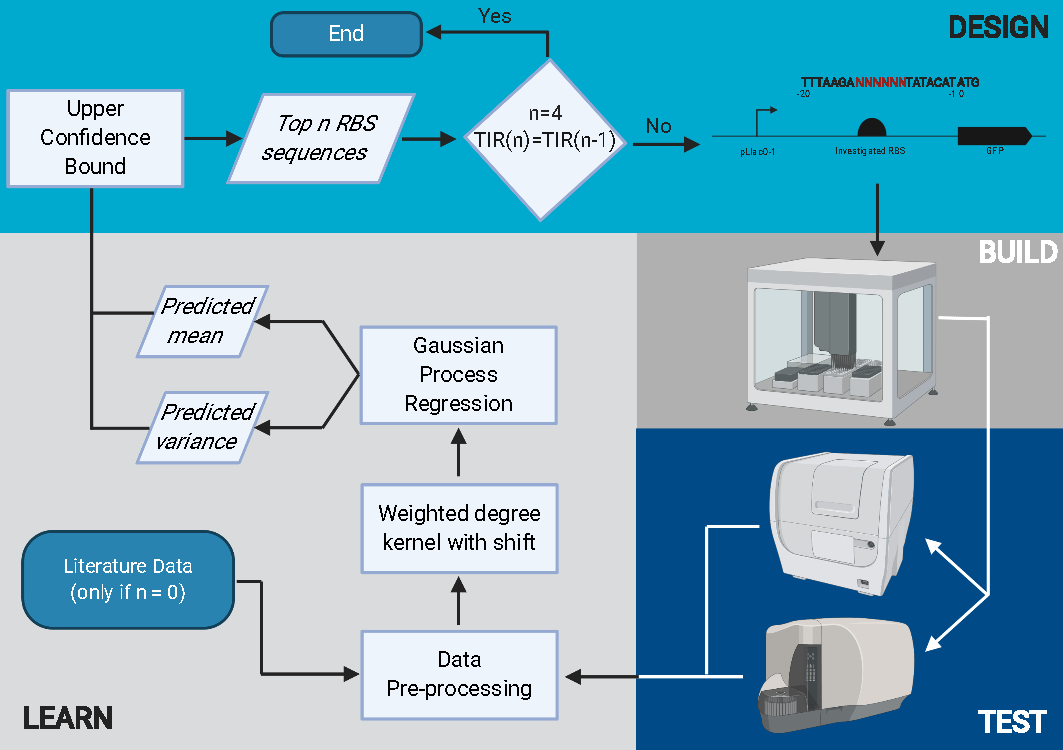
\includegraphics[scale=0.7]{plots/flowchart.pdf}
    \caption{Flowchart of machine learning based experimental design.}
    \label{fig: flowchart of machine learning based experimental design.}
\end{figure}







\section{Results}

We present our RBS-optimising DBTL workflow that uses machine learning in Section~\ref{sec:dbtl-workflow}.
In this case, the {DBTL} paradigm is applied directly to the design of the RBS part itself, rather than general strain optimisation.
Machine learning is used in two different ways: i) we show the efficacy of the ML recommendations
in the Design stage (Section~\ref{sec:ucb-results}),
and ii) we demonstrate that the ML predictions are accurate in the Learn stage (Section~\ref{sec:gp-results}).
We present our new RBS sequence library in Section~\ref{sec:characteristics-of-library} and describe some interesting
characteristics of the discovered sequences,
as well as show the effectiveness of the automated laboratory workflow.

\subsection{The experimental workflow}
\label{sec:dbtl-workflow}

Our DBTL workflow, which uses machine learning to optimise protein expression, is shown in Figure \ref{fig: Flowchart}.
Build and Test are driven chiefly by choices made by human researchers and the use of automated methods.
Machine learning algorithms are applied in Learn and Design.
In the Learn phase, we use the Gaussian Process regression algorithm to predict the TIR of RBS sequences comprising the experimental space.
In the Design phase, we use the Bandit algorithm to recommend new RBS sequences based on the predictions from Learn.\\

\begin{figure}[h]
    \centering
    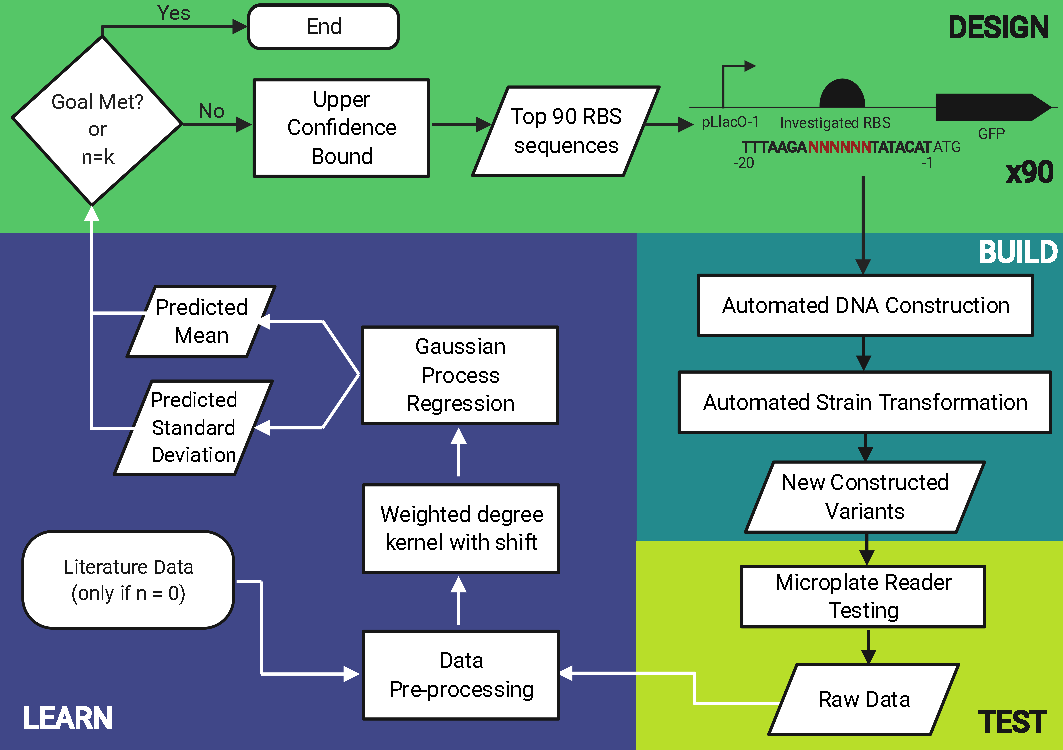
\includegraphics[scale=0.7]{plots/Main_Paper/flowchart.pdf}
    \caption{\textbf{Flowchart of the machine learning-based experimental design.} The RBS design is recommended by the Upper Confidence Bound multi-armed Bandit algorithm. After generating the recommendations, the RBSs are built and tested using automated laboratory methods allowing for rapid construction and testing at scale. Finally, the obtained results are fed back to the Gaussian Process Regression prediction algorithm in the Learn phase. n is the current design round and k is the maximum number of rounds allowed by time and/or money. In regards to the "Goal Met?" condition, the goal in our case was to find sequences with TIR significantly higher than benchmark, but the goal can be generalised to fit the requirements of the user.} 
    \label{fig: Flowchart}
\end{figure}

In our genetic design, the investigated RBS controls expression of green fluorescent protein (GFP).
By controlling expression of a fluorescent protein with the RBS we can quickly assess the perceived relative TIR by measuring fluorescence of cells harbouring the expression vector over time.
Finally, the mRNA is transcribed from an IPTG-inducible promoter pLlacO-1.
Inducible expression allows one to synchronise the start of the GFP expression in all the cultures with addition of IPTG.
Since standardisation and comparative studies should be done in as similar genetic context as possible, the design of this device has been deliberately kept simple to make such studies easier \cite{Beal2021}.\\

Our template RBS sequence is 20 base pairs (bp) long with the sequence TTTAAGA\textbf{AGGAGA}TATACAT, where the highlighted nucleotides constitute the core of the RBS.
This sequence is known to have a very high TIR in a similar context of expressing fluorescent protein and is present in the pBb series of plasmids \cite{Lee2011}.
Since this is the sequence against which new RBS sequences will be benchmarked,
we will refer to this sequence as the \textit{benchmark sequence} hereafter.
Additionally, we have experimentally confirmed that modifying the core sequence is statistically more impactful on TIR than changes made outside of it (see Figure \ref{fig:core_vs_noncore}).
This hypothesis has been built based on reported biases towards certain bases present in the core of the RBS but absent outside of it.
For example, according to \cite{SHULTZABERGER2001} there is a strong bias towards A and G bases in the core region of the RBS.
Similarly, outside of the 6 bases of the core in the wider 20 bp context of the RBS there is no significant bias towards any particular base which suggest that these bases do not contribute to the overall TIR of a given RBS. 
Focusing on the 6 to 8 bp core sequence is a common RBS design approach \cite{Jeschek2016}.
Hence, in our design, we focus on modification of the core at nucleotide positions -8 to -13 (relative to the start codon of the GFP; this is where the consensus Shine-Dalgarno AGGAGG sequence is usually found in wild type \textit{E. coli}) of the RBS and we keep other positions the same as the benchmark sequence, i.e. TTTAAGA + NNNNNN + TATACAT, where N can be any nucleotide (A, C, G, T). 
The total experimental (variant) space is then $4^6$ = 4096.

\subsection{DESIGN: Performance of the recommendation algorithm}
\label{sec:ucb-results}


The Bandit recommendations were made using the batch Upper Confidence Bound multi-armed Bandit algorithm.
In short, this algorithm is a stochastic method of probing the experimental space. 
It aims at maximising the reward (output) from testing a limited number of instances from a large pool which cannot be tested exhaustively due to limited resources (time, computational power, money).
It balances the exploration-exploitation paradigm, where exploration focuses on testing data points which maximise information gain and exploitation focuses on recommending RBSs with high predicted TIR.\\

Figure \ref{fig: Swarmplot and Quantplot}A shows the results for all the RBS groups tested experimentally.
In each experimental round, in addition to the new RBS designs, we measure the TIR of the benchmark RBS as the internal standard.
We then obtain the normalised TIR (called \textit{TIR ratio}) by taking the ratio between the raw TIR of a new design and the average TIR of benchmark sequences in each round (which are run in triplicate in each round).
Figure \ref{fig:rawswarmplots.} shows these results in terms of raw TIRs.\\

\begin{figure}[!ht]
    \centering
    \begin{subfigure}[b]{0.48\textwidth}
        \centering
        \caption{}
        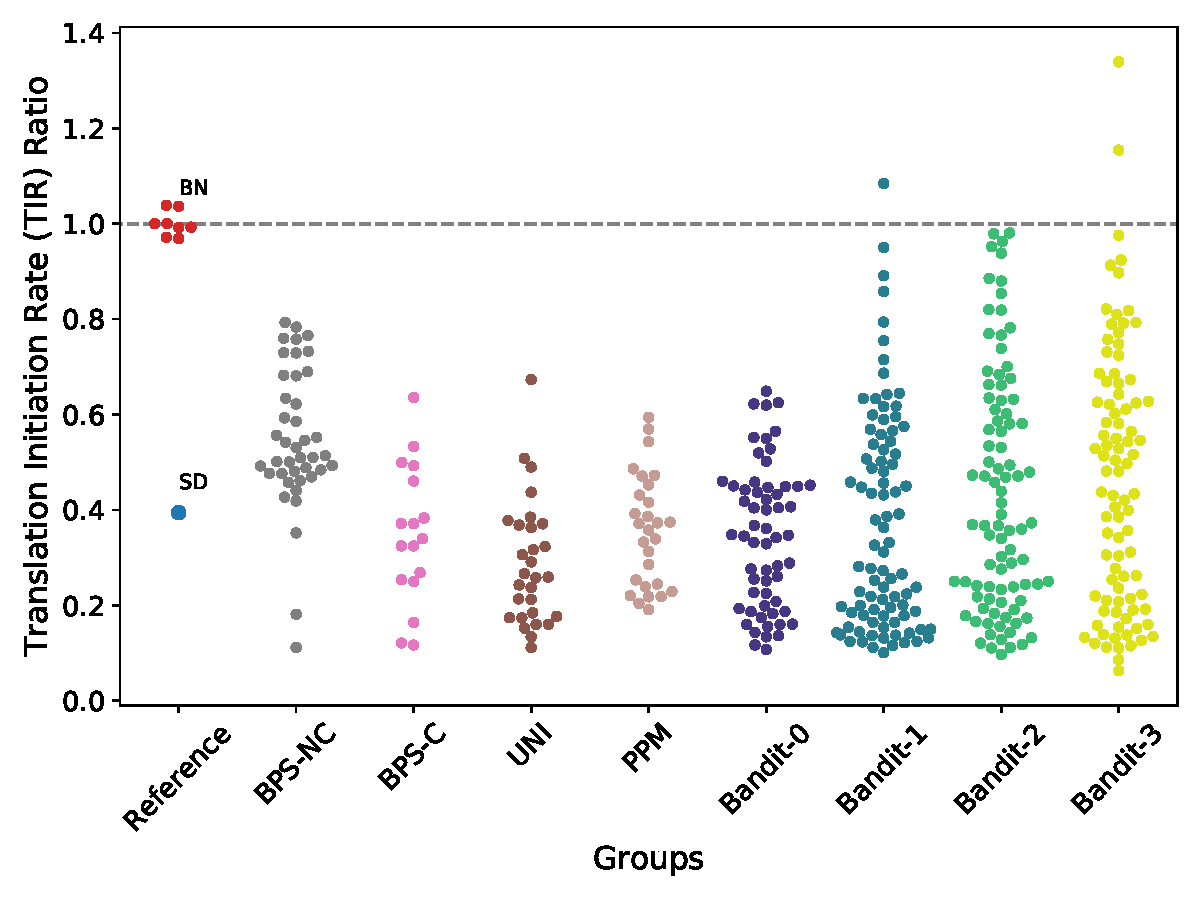
\includegraphics[scale=0.35]{plots/Main_Paper/swarmplot.pdf}
    \end{subfigure}
    % \hfill
    \begin{subfigure}[b]{0.25\textwidth}
        \centering
        \caption{}
        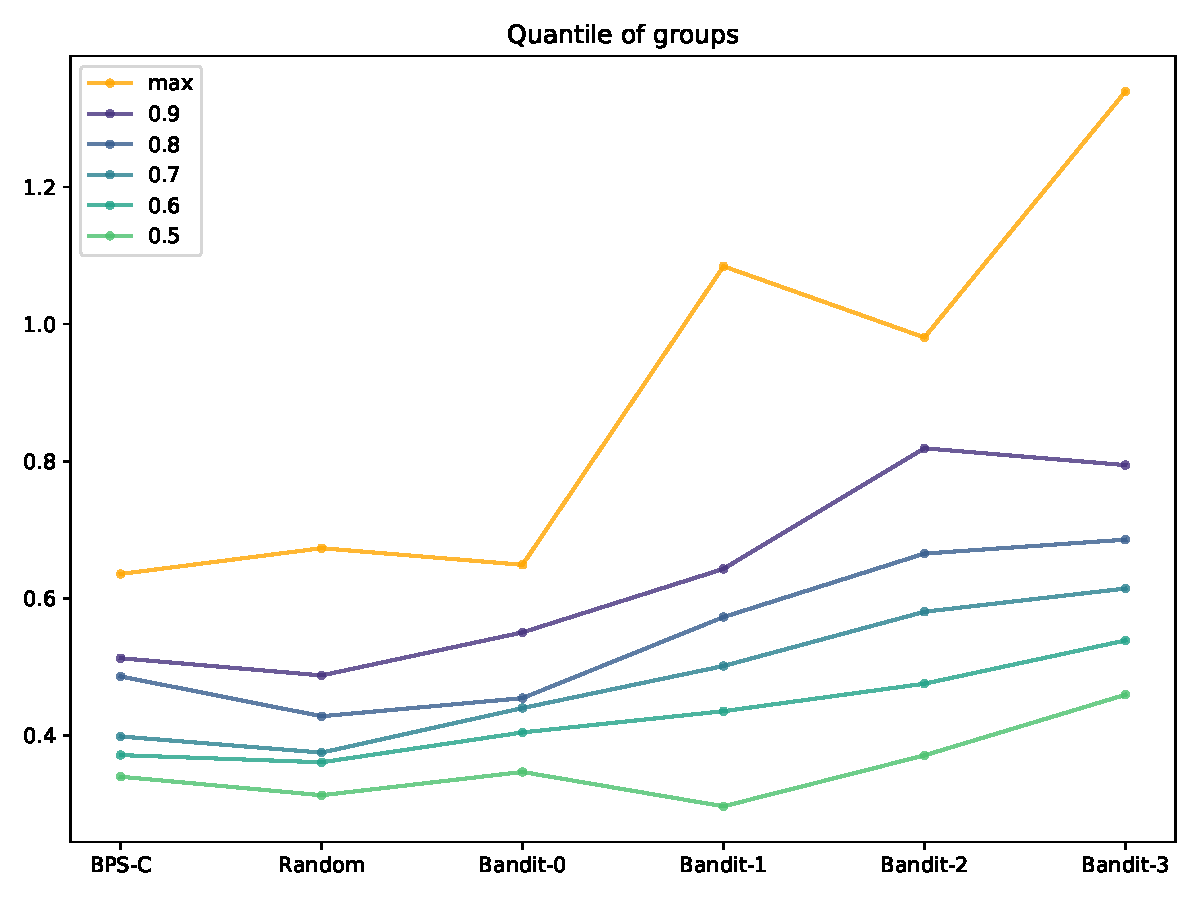
\includegraphics[scale=0.35]{plots/Main_Paper/quantplot.pdf}
    \end{subfigure}
    % \hfill
    \begin{subfigure}[b]{0.25\textwidth}
        \centering
        \caption{}
        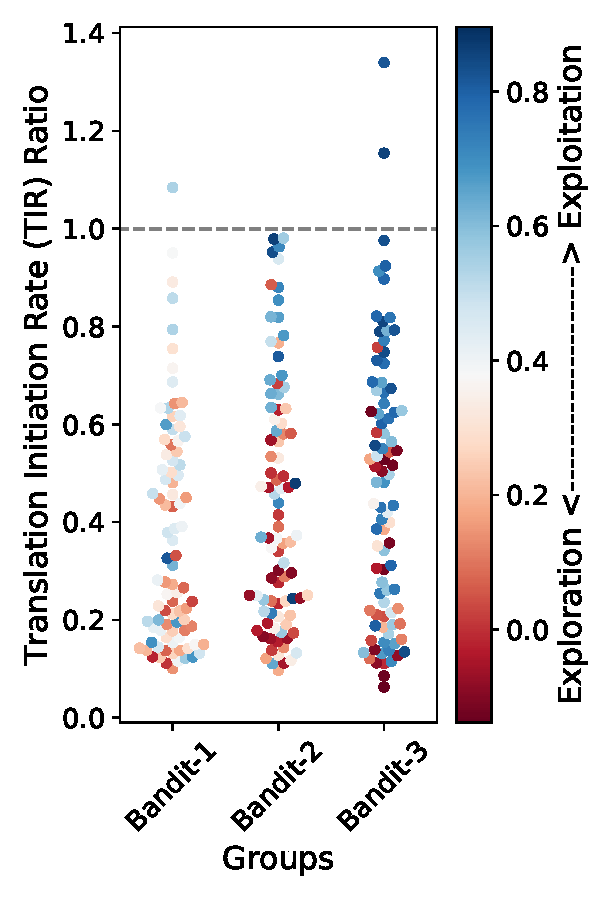
\includegraphics[scale=0.35]{plots/Main_Paper/swarmplot_proj.pdf}
    \end{subfigure}
    \begin{subfigure}[b]{0.48\textwidth}
        \centering
        \caption{}
        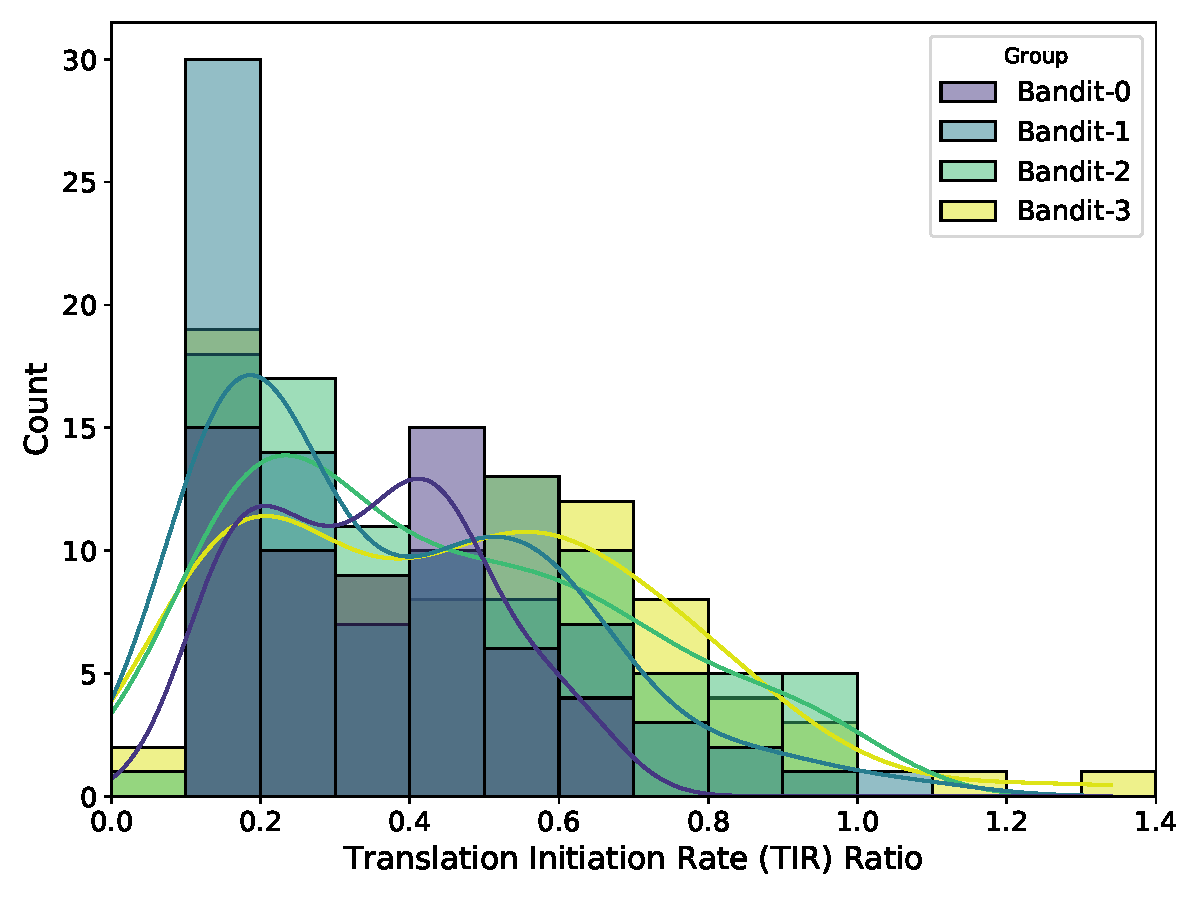
\includegraphics[scale=0.4]{plots/Main_Paper/histogram.pdf}
    \end{subfigure}
    \begin{subfigure}[b]{0.48\textwidth}
        \centering
        \caption{}
        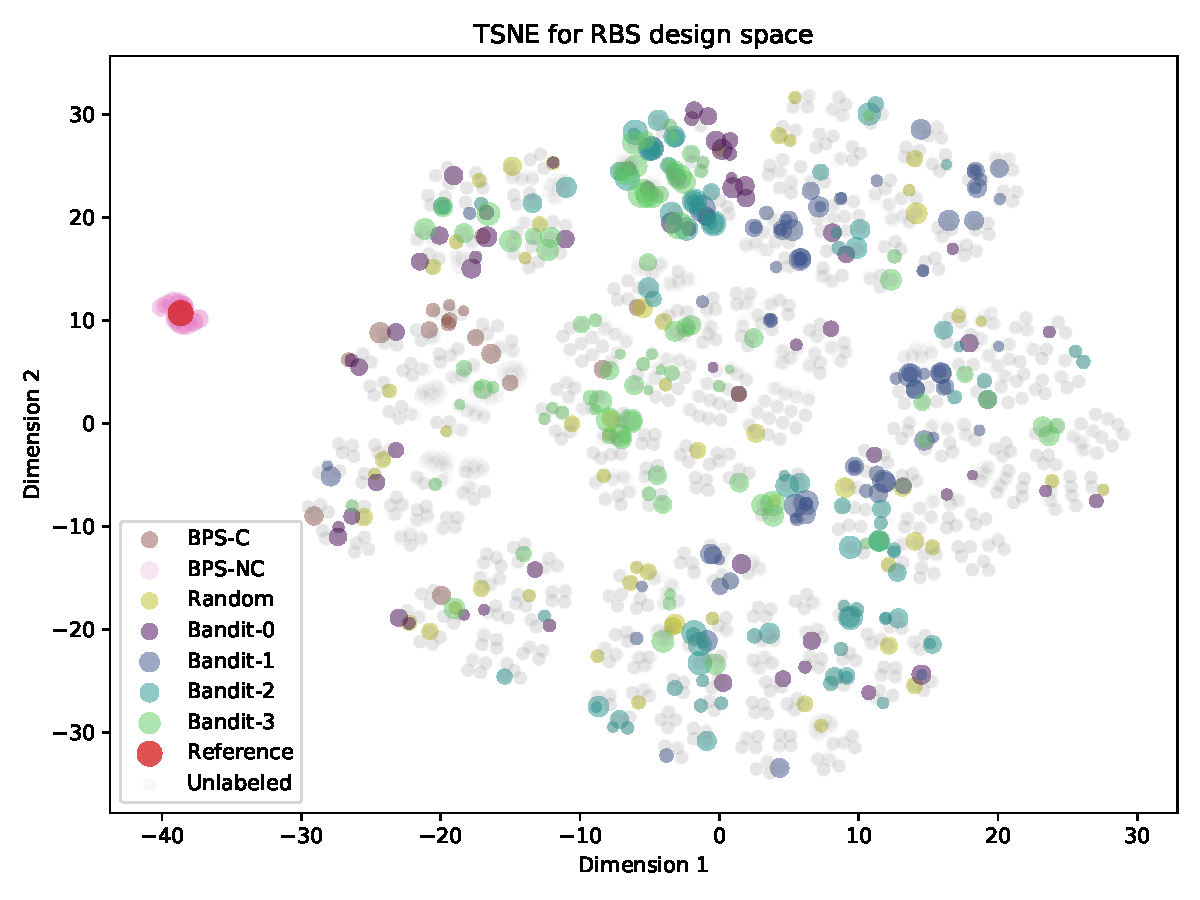
\includegraphics[scale=0.42]{plots/Main_Paper/tsneplot.pdf}
    \end{subfigure}
    % 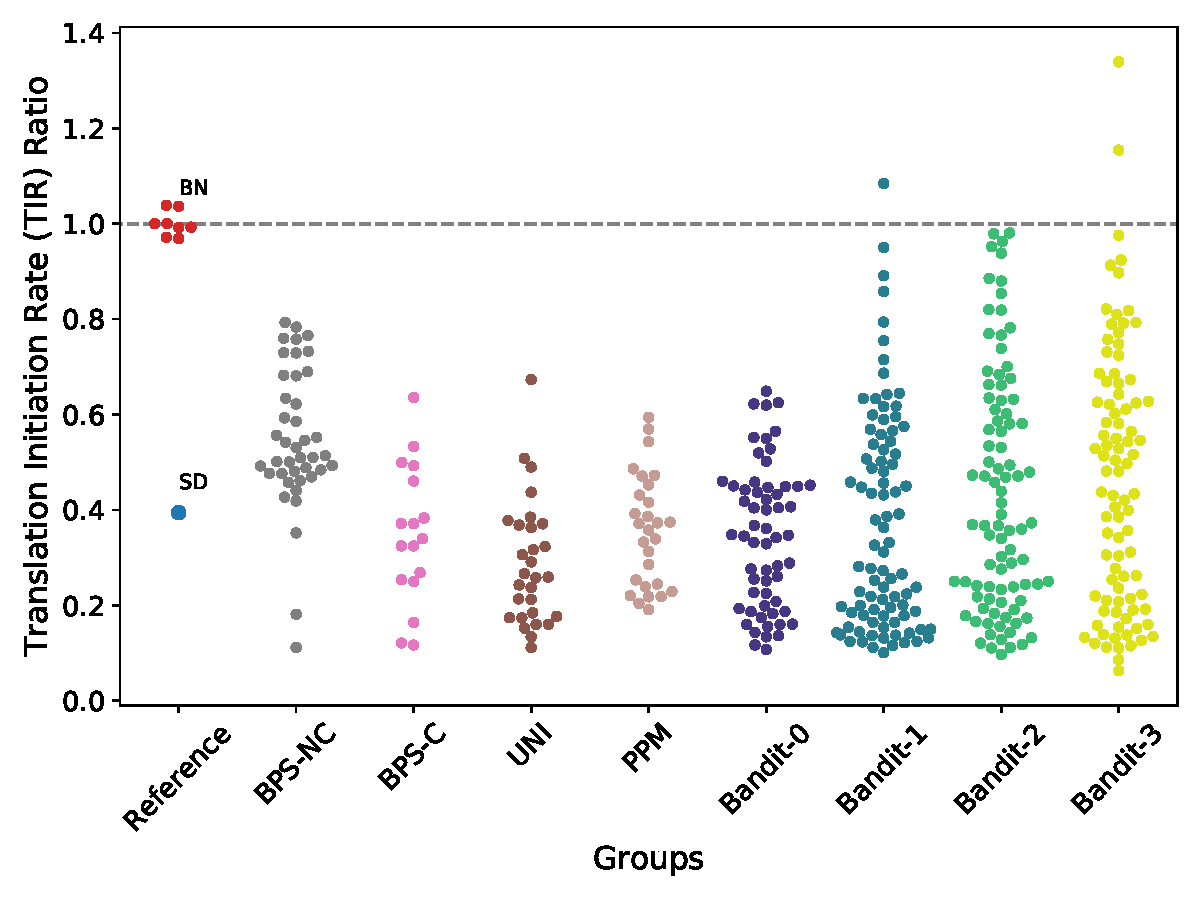
\includegraphics[scale=0.3]{plots/Main_Paper/swarmplot.pdf}
    % 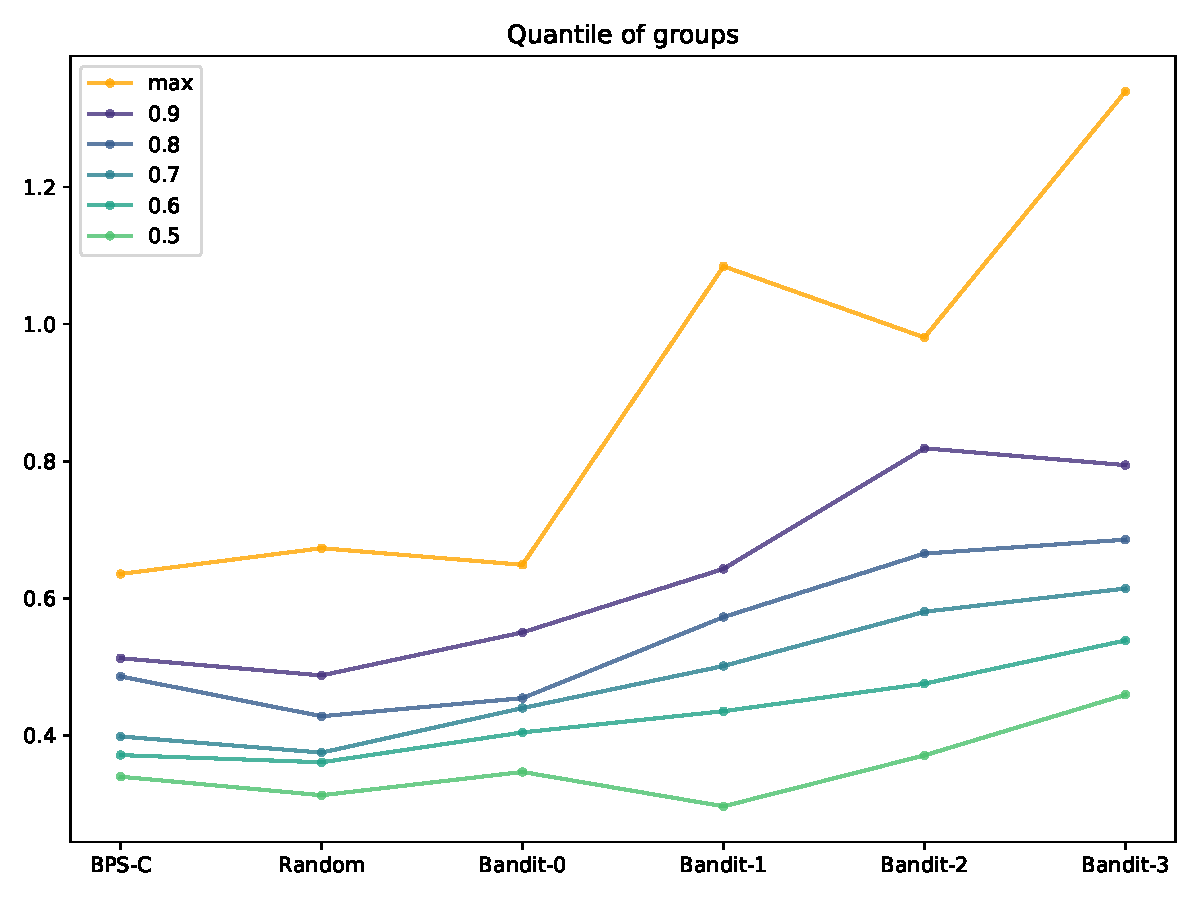
\includegraphics[scale=0.3]{plots/Main_Paper/quantplot.pdf}
    % 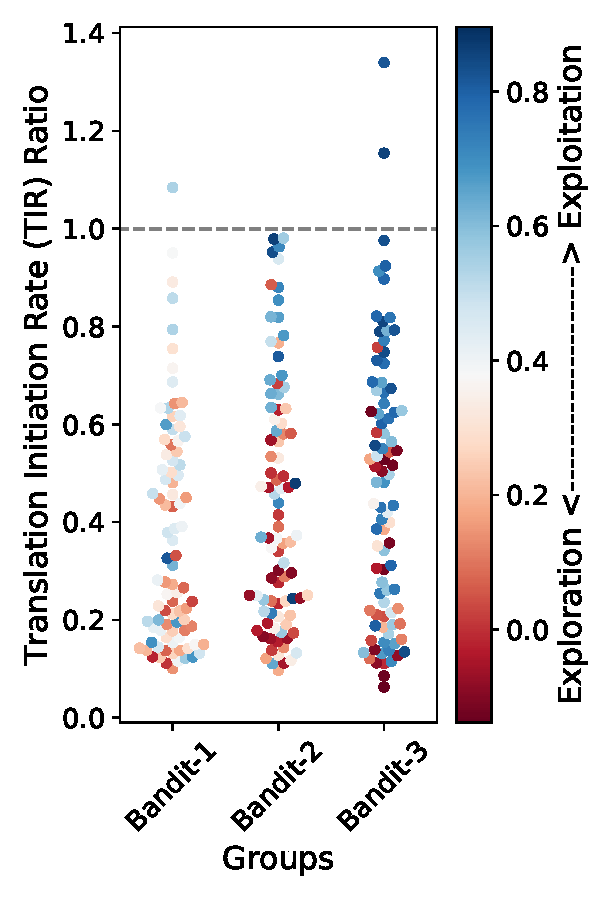
\includegraphics[scale=0.3]{plots/Main_Paper/swarmplot_proj.pdf}
    % 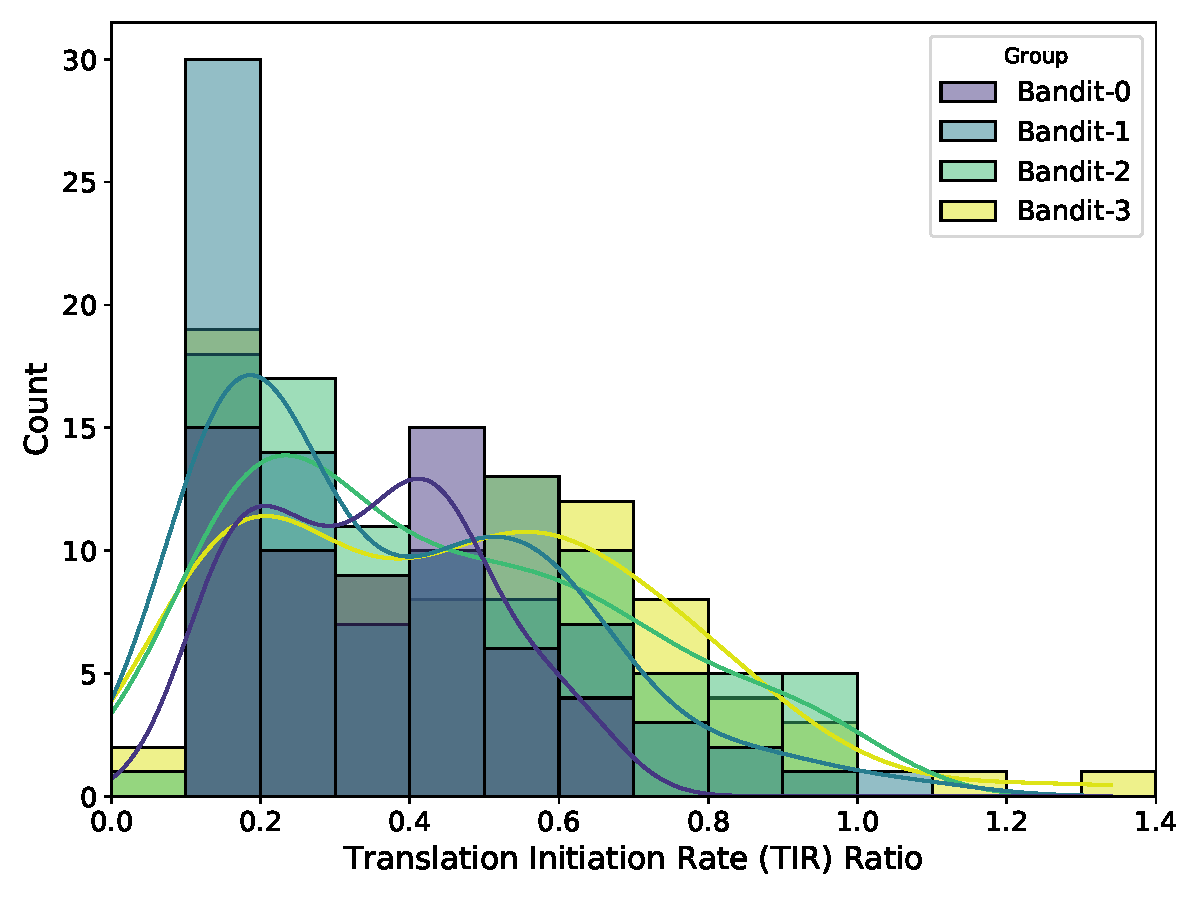
\includegraphics[scale=0.3]{plots/Main_Paper/histogram.pdf}
    % 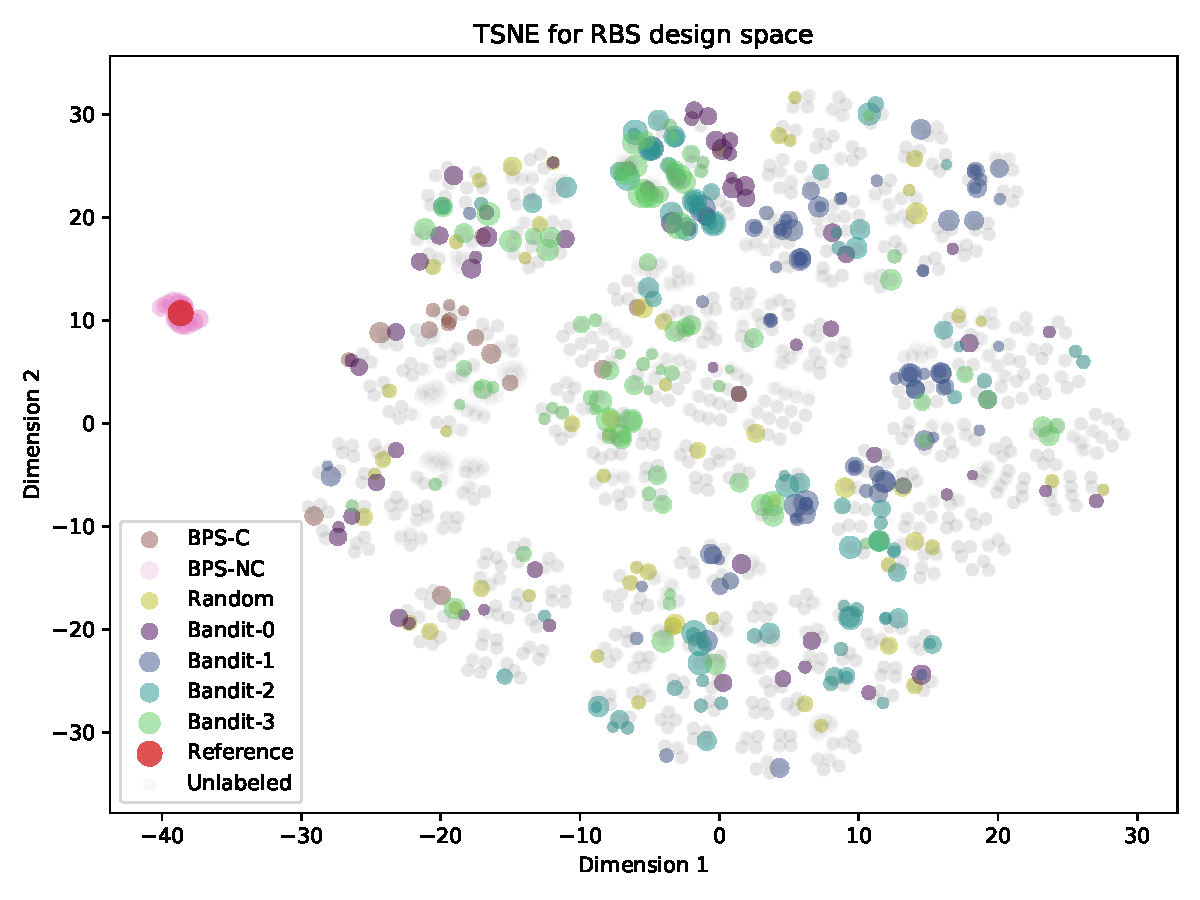
\includegraphics[scale=0.4]{plots/Main_Paper/tsneplot.pdf}
    \caption{
    \textbf{TIRs of RBS groups examined in this study.}
    \textbf{A)} Swarm plot showing the obtained TIRs divided into RBS groups.
    BPS-NC: base-by-base changes in the non-core region. 
    BPS-C: base-by-base changes in the core region. 
    UNI: Randomly generated sequences with uniform distribution. 
    PPM: Randomly generated sequences with distribution following the Position Probability Matrix for all natural RBS in \emph{E. coli}. 
    Bandit-0/1/2/3 - Bandit algorithm generated results for Round 0, 1, 2 and 3 respectively.
    SD - Shine-Dalgarno sequence.
    Dashed line is set to 1 and represents the averaged benchmark sequence TIR for that group. 
    BN - benchmark sequences for all plates. 
    (not all are exactly 1 due to them being shown as separate samples rather than per round averages.)
    \textbf{B)} Line plot showing TIR obtained in a given quantile (Q) of results divided into groups as in A).
    % save the random groups which were shown together due to similar distributions.
    UNI and PPM are merged into Random group and BPS-NC is not shown due to changes being made outside the core in that group.
    \textbf{C)} Exploitation v.s. Exploration for Bandit 1-3. Blue-hued points represent exploitation, those hued red represent exploration.
    \textbf{D)} Histogram with kernel density estimations (KDE) showing distributions of TIRs for Bandit groups.
    \textbf{E)} t-SNE plot showing the relative distances between sequences in our design spaces as calculated by our kernel function (weighted degree kernel with shift). 
    The area of the circle corresponds to the experimentally-obtained TIR value.
    The TIR results in all subplots are shown normalised to the respective benchmark sequence sample which acts as internal standard; the TIR of a given RBS is divided by TIR of the benchmark RBS run in the same plate. }
    \label{fig: Swarmplot and Quantplot}
\end{figure}

To generate the data set from which the algorithm would learn, we decided to characterise a total of 450 RBS variants, little over 10\% of the whole experimental space. 
To fit our automated workflow, we divided the 450 variants into batches of 90, split into 4 design rounds.\\

In the zeroth Round we tested two batches of designs, giving a total of 180 variants split as below: 

\begin{itemize}
    \item BPS-NC and BPS-C group: 60 RBS sequences which are subsequent single nucleotide variations of all 20 nucleotides of the original, benchmark sequence. This batch is designed to show us influence of such single nucleotide changes on the overall performance of the RBS and the potential impact of changes made beyond the core part (see Supplementary Figure \ref{fig:core_vs_noncore}).
    % \mengyan{put it in main paper?}
    \item UNI group: 30 RBS sequences that were uniformly randomised, i.e. equal probability of choosing any nucleotide for each position. This group shows the performance of RBSs generated randomly.
    \item PPM group: 30 RBS sequences randomised based on the position probability matrix (PPM) generated from all the naturally-occurring RBS sequences in  the \emph{E. coli} genome \cite{barrick1994quantitative}. This group shows the performance of RBSs generated randomly, but following the natural nucleotide distribution.
    \item Bandit-0: 60 RBS sequences recommended by our implementation of the recommendation algorithm based on a data set obtained from literature \cite{jervis2018machine}, which contains 113 non-repeated records for 56 unique RBS sequences with their respective TIRs.
    This data set has been used due to the perceived similarity of its goal to that of this work - prediction of TIR based on phenotypic output.
\end{itemize}

In the subsequent 3 rounds, with one batch each, all 90 designs were generated using our machine learning algorithm based on the data obtained from the previous rounds (these groups are called Bandit 1 to 3 respectively).\\

All Round 0 groups (BPS-NC, BPS-C, UNI, PPM, Bandit-0) performed worse than our benchmark sequence in terms of TIR. 
The best-performing group was the BPS-NC, which is explained by the relatively small impact on the TIR of changes made outside the RBS core. 
The Bandit-0 group's performance is similar to randomly generated designs, despite being machine learning-driven, due to being trained on approximate data.
% \hl{These results show that generating a strong RBS sequence by random mutations is a non-trivial task, when the tested data set is relatively small.}\\
Starting from Round 1, where the prediction and recommendation algorithms were fed data from Round 0, the results improved significantly, with a number of sequences performing better than the consensus Shine-Dalgarno sequence and in one case, better than the benchmark (by 8\%).
In Round 2 we observed further improvement by obtaining more sequences with TIRs similar to our benchmark sequence.
Finally, in Round 3 the algorithm identified two sequences that were 34\% and 15\% stronger than the benchmark sequence.\\

In summary, out of 450 tested sequences, around 40\% (BPS-NC, BPS-C, UNI, PPM) were created through some kind of sequence randomisation. Out of these randomised sequences, only a few got close to the benchmark sequence's TIR and were still 20\% weaker than it is (Figure 3A). In fact, these 80\% TIR ratio sequences were created by randomising the sequence outside of the core RBS region (BPS-NC), which was statistically shown not to be significantly impactful on the TIR (see Supplementary Figure S1 and, for example, work by \mbox{\textcite{Jeschek2016}}). More representative would be sequences from other random groups (BPS-C, UNI, PPM), from which the best sequence achieved only about 65\% of the benchmark TIR. 
These results show that generating a strong RBS sequence by random mutation is a non-trivial task, when the tested data set is relatively small.
Contrasted with this, non-randomized, our Bandit-driven design batch gave much better results, with RBSs getting close to benchmark performance and even exceeding it.\\

Figure \ref{fig: Swarmplot and Quantplot}B shows the same results but divided into quantiles where the specific point for a given group shows the highest TIR for that quantile.
The gradual increase for all quantiles can be observed for all Bandit groups, suggesting that the algorithms have a better understanding of the experimental space given more data.
The decreased result in the 0.9th quantile compared to the maximum value for the Bandit 3 group can be attributed to the increased emphasis on exploitation that has been set for that round compared to others.
We see this effect in Figure \ref{fig: Swarmplot and Quantplot}C (with details shown in Figure  \ref{fig:exploitationvsexplorationdetail}), where we coloured the data points for Bandit 1-3 groups according to their relative exploration - exploitation affinity.
Those with a high predicted mean are coloured blue and represent exploitation, those coloured red are with high predicted uncertainty and represent exploration.
\hl{Since we expect that an RBS sequence chosen at random will have low TIR
(as shown by UNI and PPM), this implies that most of the exploration will result in low TIR.
Our results confirm that
RBSs with high TIRs tend to come from exploitation of the design space,
whereas the exploration points give relatively low TIRs. Note that the exploration is necessary to expand our knowledge of unknown parts of the design space.}\\

Figure \ref{fig: Swarmplot and Quantplot}D shows the TIRs of RBSs tested in the Bandit groups divided into bins with width equal to a TIR ratio of 0.1.
KDE plots have been overlaid to depict the calculated density for each group.
The increase in prevalence of later Bandit groups in the higher bins is evident, especially for Bandit 2 and 3, constituting the bulk of results in the $>0.8$ TIR ratio bins.
Notably, the distributions calculated for all the groups are bimodal - we discuss the possible reasons for that later in the text.\\


In Figure \ref{fig: Swarmplot and Quantplot}E we show a t-distributed stochastic neighbour embedding (t-SNE) \mbox{\cite{tsne2008}} plot depicting the experimental space.
Each RBS is located on the plot according to its distance from other RBSs as calculated by our weighted degree kernel with shift (see Section \mbox{\ref{sec: method prediction with kernel}}).
The RBSs recommended by Bandit groups have covered the majority of the design space. 
Additionally, a number of clusters were especially targeted by our recommendation algorithm.
For example, the circled clusters labelled as "G-Rich Clusters" have been actively recommended by the algorithm.
More specifically, sequences with 4 or more guanines in any position constituted 10\% of the randomly selected sequences and 5, 9, 16 and finally 25\% in each of the 4 Bandit guided batches respectively.

\subsection{LEARN: Prediction of RBS performance}
\label{sec:gp-results}


Figure \ref{fig: Scatterplot} shows how our implementation of the Gaussian Process algorithm performed in terms of predictions in each round. 
As expected, the predictions in Round 0 were poor due to use of approximate data. 
The predictions improved for the subsequent rounds, from R\textsuperscript{2} (coefficient of determination) of 0.067 for Round 0 to R\textsuperscript{2} of 0.213 for Round 3.
Similarly, the Spearman correlation coefficient rose from 0.269 for Round 0 to 0.546 for Round 3.
Figure \ref{fig:scatter abc1 TT.} shows the performance of predictions for individual rounds.\\

The obtained values of the coefficient of determination and Spearman correlation coefficient are influenced by a number of factors.
The primary one is our choice of the exploration-exploitation balance.
In each round, we select a number of data points for exploration, which means that when tested, they have a high chance of having a experimentally-obtained mean different from what was predicted, thus decreasing the R\textsuperscript{2} values.
However, this is very useful information for future predictions as it allows us to understand the underlying space better.
The effect of better exploration of the space is the ability to find high TIR RBSs even with relatively low R\textsuperscript{2} values.\\


\begin{figure}[!ht]
    \centering
    \begin{subfigure}[b]{0.49\textwidth}
        \centering
        \caption{}
        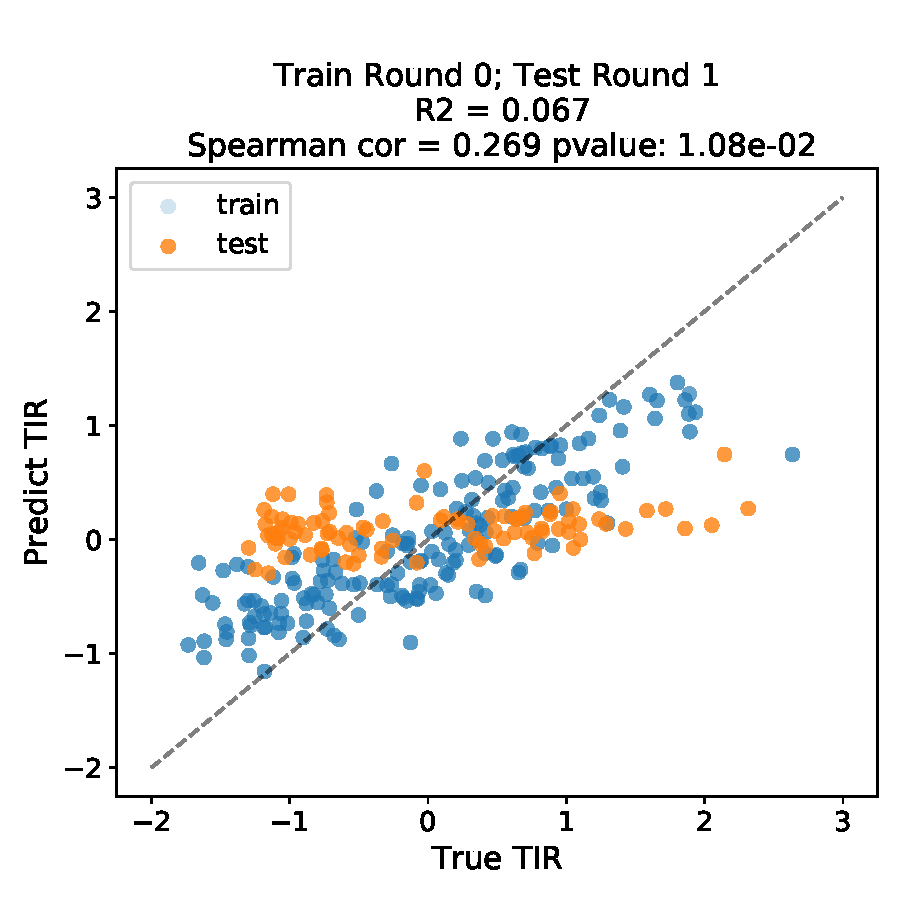
\includegraphics[scale=0.4]{plots/Main_Paper/scatter_abc1_FF_0.pdf}
    \end{subfigure}
    % \hfill
    \begin{subfigure}[b]{0.49\textwidth}
        \centering
        \caption{}
        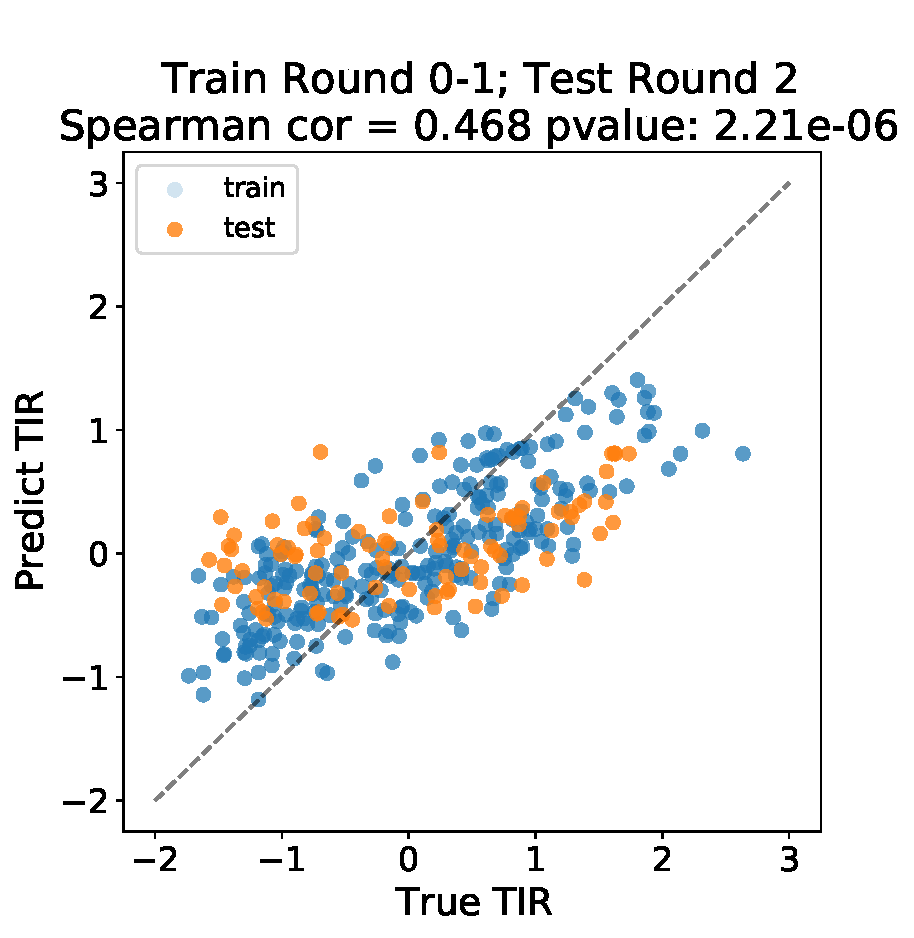
\includegraphics[scale=0.4]{plots/Main_Paper/scatter_abc1_FF_1.pdf}
    \end{subfigure}
    % \hfill
    \begin{subfigure}[b]{0.49\textwidth}
        \centering
        \caption{}
        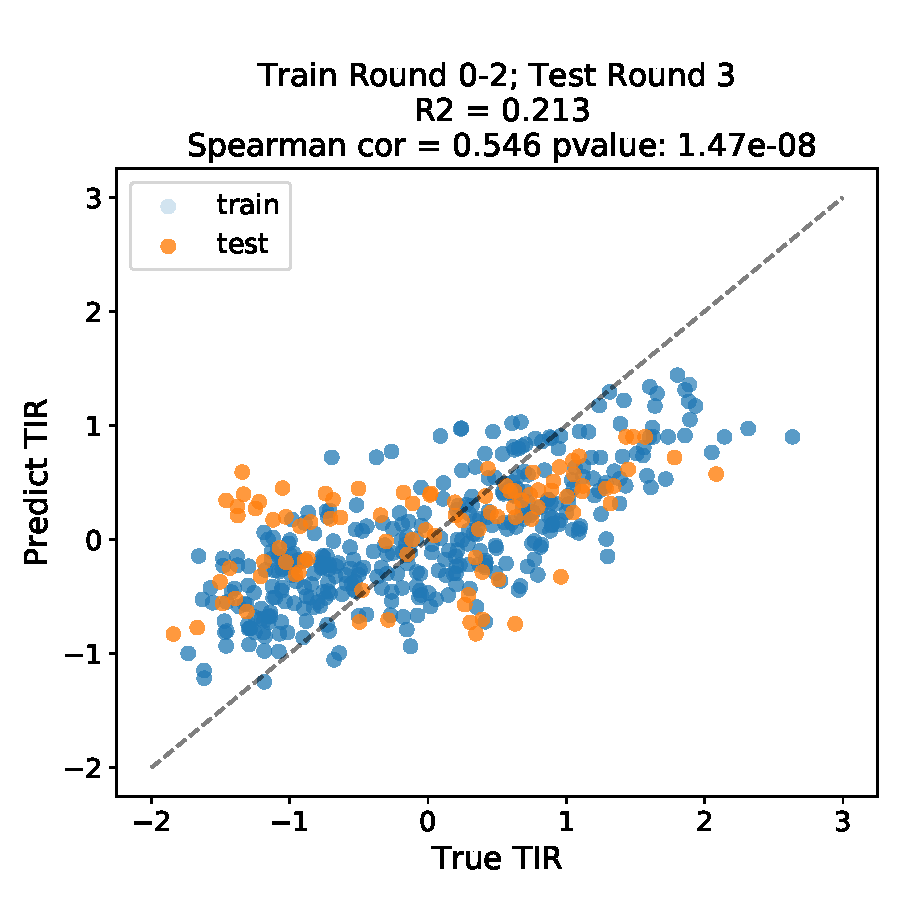
\includegraphics[scale=0.4]{plots/Main_Paper/scatter_abc1_FF_2.pdf}
    \end{subfigure}
    \begin{subfigure}[b]{0.49\textwidth}
        \centering
        \caption{}
        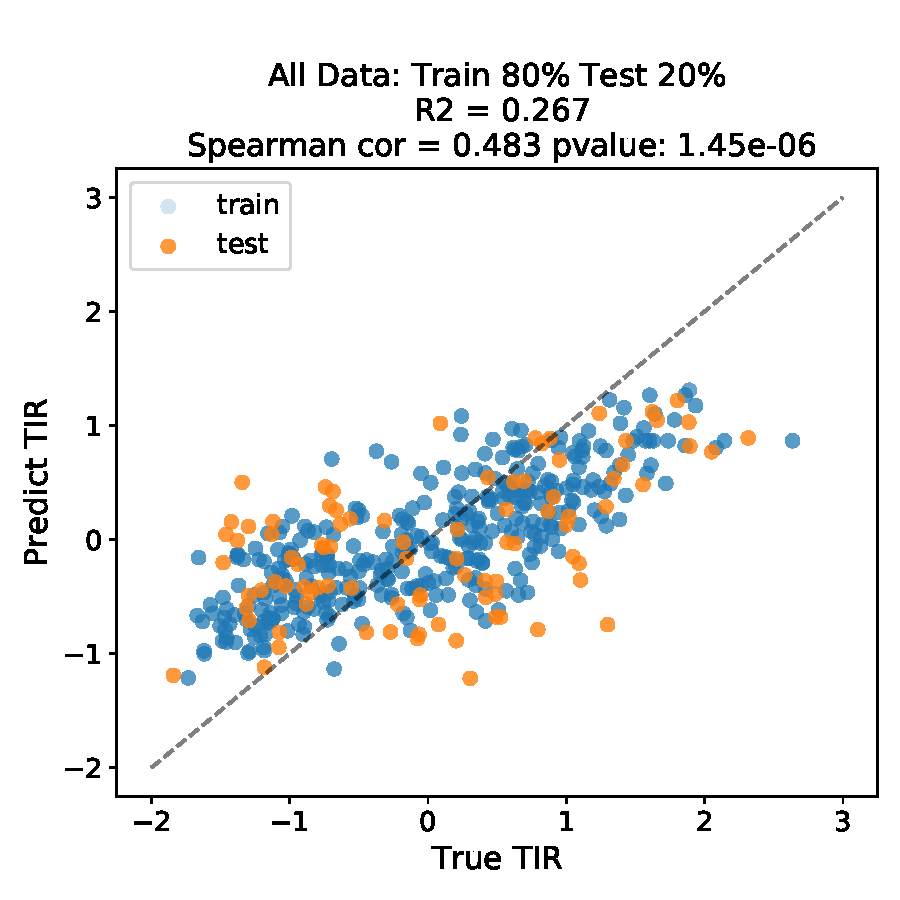
\includegraphics[scale=0.4]{plots/Main_Paper/scatter_abc1_FF_3.pdf}
    \end{subfigure}
    \caption{\textbf{Performance of the prediction algorithm (no kernel normalisation)}. The scatter plots A-D show the performance of our prediction algorithm calculated after each round.
    Note that the TIR values are normalised according to the standardisation described in section \ref{sec: method data pre-procesing}, which is different from the TIR ratio reported in Figure \ref{fig: Swarmplot and Quantplot}.
    The $R^2$ value and Spearman correlation coefficient (with corresponding p-value) are provided for each plot.
    The p-value here is for the null hypothesis stating that two sets of data are uncorrelated.
    }
    \label{fig: Scatterplot}
\end{figure}

\subsection{BUILD \& TEST: Characteristics of the tested sequences}
\label{sec:characteristics-of-library}

% Taken together, our data can be viewed as a reliable (low coefficients of variation) and extensive (high number of entries compared with widely used iGEM RBS collections, for example \cite{IGEM}) library of RBS sequences for \emph{E. coli}, some characteristics of which are shown in Table 1.\\

\hl{We present some important characteristics of the tested RBSs in Table 1}.
Figure \ref{fig:Library characteristics}A shows the sequence logo calculated for the Top 30 sequences (Figure \ref{fig: All_logo} shows the logo generated for all tested sequences).
It is generally understood that guanine-rich sequences promote strong transcription.
This expected bias towards guanine is clearly visible for all positions in our Top 30 RBSs.
This result combined with the Bandit algorithm's bias towards the G-rich cluster shown in Figure \ref{fig: Swarmplot and Quantplot}D reinforces the notion that our algorithm successfully identified G-rich sequences as the ones with high TIR probability.\\

\begin{figure}[!t]
     \centering
     \begin{subfigure}[b]{0.49\textwidth}
         \centering
         \caption{}
         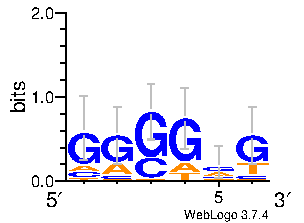
\includegraphics[scale=1.2]{plots/Main_Paper/TOP30_logo.pdf}
     \end{subfigure}
     \hfill
     \begin{subfigure}[b]{0.49\textwidth}
         \centering
         \caption{}
         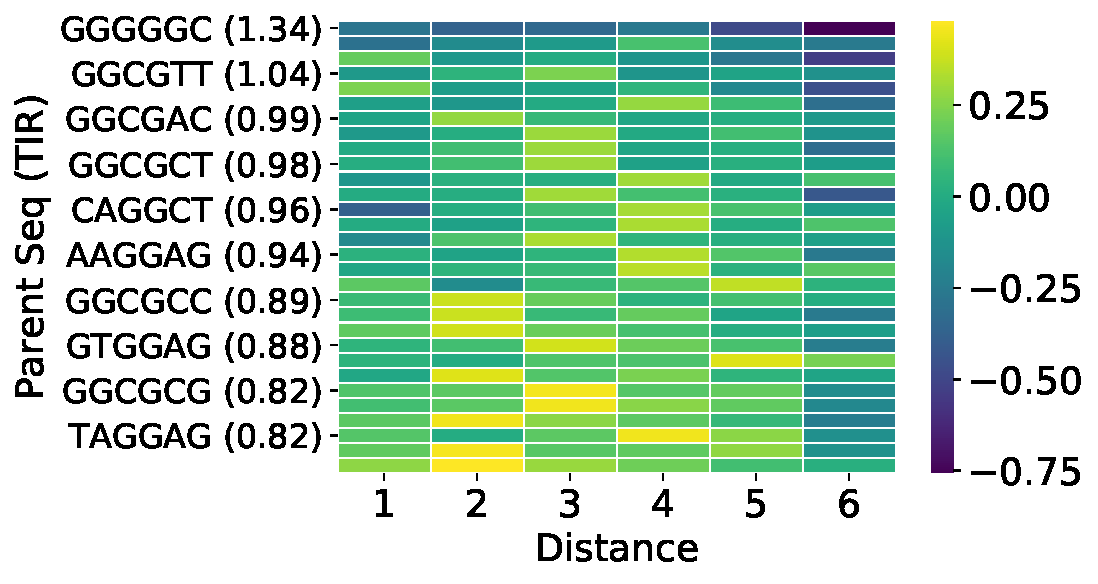
\includegraphics[scale=0.43]{plots/Main_Paper/heatmap.pdf}
     \end{subfigure}
     \caption{\textbf{Characteristics of strong RBSs.} A) Sequence logo calculated for the Top 30 tested sequences. B) Heatmap showing the edit (Hamming) distance required for positive change in TIR for RBSs with high and medium TIRs. The temperature scale shows the difference between a given RBS on the y-axis and the RBS with the strongest TIR at the given distance. Every second RBS is labelled for increased legibility.}
     \label{fig:Library characteristics}
\end{figure}

\begin{table}[!h]
\centering
\begin{minipage}[c]{0.6\textwidth}
\centering
\begin{tabular}{|c|c|}
\hline
\textbf{Characteristics of the library}                                                       & \textbf{Statistics} \\ \hline
Total experimental space                                                                      & 4096                \\ \hline
Planned constructs                                                                            & 450                 \\ \hline
Successfully constructed                                                                      & 445                 \\ \hline
Sequences with CV\textless{}40\%                                                              & 79\%                \\ \hline
Sequences with CV\textless{}20\%                                                              & 27\%                \\ \hline
\begin{tabular}[c]{@{}c@{}}Efficiency of Bandit design \\ (compared with random)\end{tabular} & 2                   \\ \hline
Raw TIR range                                                                                     &      [4.93, 105.38]               \\ \hline
TIR ratio range                                                                                     &      [0.06, 1.34]               \\ \hline
\end{tabular}
\end{minipage}
\begin{minipage}[c]{0.38\textwidth}
\centering
% Please add the following required packages to your document preamble:
% \usepackage[table,xcdraw]{xcolor}
% If you use beamer only pass "xcolor=table" option, i.e. \documentclass[xcolor=table]{beamer}
\begin{tabular}{|c|c|}
\hline
\textbf{Top RBS Core} & \textbf{TIR Ratio} \\ \hline
GGGGGC                & 1.34             \\ \hline
GGGGGT                & 1.15             \\ \hline
GGCTAT                & 1.08              \\ \hline
\textbf{AGGAGA}                & 1                  \\ \hline
GGCGTT                & 0.98            \\ \hline
GGGGGG                & 0.98             \\ \hline
GGCGAC                & 0.98             \\ \hline
CAGGAG                & 0.96             \\ \hline
GGCGAG                & 0.95             \\ \hline
\textbf{AGGAGG}       & 0.39            \\ \hline
\end{tabular}
\end{minipage}
\caption{\textbf{Characteristics of the library.}
Left table presents some of the characteristics of our library.
Right table presents 10 RBS sequences with their corresponding TIR ratios; the first 9 are the strongest sequences including the benchmark sequence (AGGAGA) and the last is the Shine-Dalgarno sequence (AGGAGG).
CV is coefficient of variation (standard deviation (STD) of a sample divided by its mean; see details in Figures \ref{fig: SDhist} and \ref{fig:variation of biological replicates}).
Efficiency of the Bandit design is calculated by dividing the highest TIR found using machine learning by the highest TIR found using random sequence generation.}
\end{table}

Another interesting characteristic uncovered by our research is the perceived editing distance between two sequences required for  improvement in the TIR when the given RBS' TIR is already high.
We define the edit distance as Hamming distance, that is, how many positions have to be changed to get from one sequence to the other (Hamming distance of 0 means that the sequences are identical and 6 means that they are two completely different sequences).
Figure \ref{fig:Library characteristics}B shows the edit distance is required for positive change in TIR for an RBS with TIR $>0.75$.
For RBSs with high TIRs ($>1$), the minimum distance that is required to increase the TIR is 2, with edit distances between 2 and 5 giving similar results.
For RBSs with medium TIRs ($<1$), a distance of 1 is enough to produce a meaningful increase in TIR.

This means that as the TIRs of examined RBSs increase, exploring sequences which are more dissimilar to the current candidates tends to give more meaningful improvement. 
As long as this does not impact targeted methods like machine learning-guided design, it does imply that the low rate of natural mutations will be very slow to explore more dissimilar sequences on such a short distance \cite{Lee2012}, which indicates that methods like Adaptive Laboratory Evolution may not be able to find very strong RBSs with a limited budget.  
In other words, because the examined sequence is relatively short (6 bp in a wider 20 bp context) the time required to accumulate 2 or more changes in the RBS region required for meaningful increase in TIR might be prohibitively long.
In such cases, a directed process, like the one described here, should be strongly encouraged.
This observation is in line with approaches seen in other disciplines, e.g. protein engineering, where more directed changes yield better results than wide random changes \cite{Jackel2008}.\\

\hl{Finally, while our strong sequences showed some affinity towards the anti-sense sequence of the ribosome known to bind to RBS, they did not show any obvious secondary structures that could explain their TIRs} (see Figure \ref{fig:structures}).
This result combined with the unexpectedly bimodal nature of KDEs in Figure \ref{fig: Swarmplot and Quantplot} reinforces the notion, based on the previously reported literature \cite{Saito2020,EspahBorujeni2016}, that there may be a number of different mechanisms governing the probability of effective RBS-ribosome binding.\\



\section{Discussion and Conclusion}

In this work, we have shown how machine learning and high-throughput, automated laboratory methods can be jointly applied to efficiently generate a library of small parts, in this case bacterial RBSs. 
We have used Gaussian Process regression to predict the TIR function to be optimised and an Upper Confidence Bound multi-armed Bandit algorithm to recommend sequences to be tested.
To represent RBSs and capture the similarities between them, we chose to use the Weighted Degree Kernel with Shift method, which fits well into our prediction method.
In building and testing, we have performed the bulk of our experiments using automation to increase their speed, reliability and reproducibility.
By using our workflow and testing only 450 RBS variants, we have designed and experimentally-validated RBSs with high translation initiation rates equalling or exceeding the currently known strong RBSs \hl{in this context} by up to 34\%.
Furthermore, we have generated an extensive library of diverse RBSs that can be used \hl{as a basis} in future studies.\\

In our work we have focused on maximising the TIR of the RBS, by gradually moving our emphasis from exploration to exploitation as we progressed through the design rounds.
This approach may have to be modified in more complex cases, especially involving multi-gene metabolic engineering since maximising expression of genes would most probably result in excessive metabolic burden.
This change could be achieved within the Bayesian optimisation framework by changing the objective of the algorithm to maximising the range of the black-box function, or identifying the part of function above a threshold \mbox{\cite{gotovos2013active}}, or combining different goals into a multi-objective method, for example \mbox{\cite{shu2020new}}.\\
% \hl{
% While we focus our optimisation framework on the RBS optimisation task, our framework has good potential to be generalised to multi-gene pathway design, as reviewed by \mbox{\textcite{LAWSON2021}} and proposed by \mbox{\textcite{hamedirad2019towards}}. For example, the optimisation goal can be adjusted to address combinatorial optimisation for multi-gene and RBS scenarios; since this would be a large-scale data task, the current Gaussian Process Regression (GPR) prediction model could be updated to a deep GPR approach and the current Bandit algorithm could be optimised towards querying large design space to reduce computational complexity \mbox{\cite{shahriari2015taking}}.  
% }

It is important to make a distinction between works focusing on the part itself like \mbox{\textcite{Hollerer2020}} and works where the part is optimised with a wider goal of strain optimisation like in \mbox{\textcite{Jervis2019}}.
The part-centric optimisation, like the one considered in this paper, is an important task in synthetic biology because metabolic pathways are made up of individual parts and understanding their performance in separation allows for better strain design. 
While we focus our optimisation framework on the RBS optimisation task, this framework has good potential to be generalised to multi-gene pathway design as reviewed by \mbox{\textcite{LAWSON2021}} and proposed by \mbox{\textcite{hamedirad2019towards}}. 
For example, the optimisation goal can be adjusted to address combinatorial optimisation for multi-gene and RBS scenarios; since this would be a large-scale data task, the current Gaussian Process regression prediction model could be updated to a deep Gaussian Process regression approach and the current Bandit algorithm could be optimised towards querying large design space to reduce computational complexity \mbox{\textcite{Shahriari2016}}.  
\\

Our approach has shown that machine learning is able to correctly detect and exploit rules of biological design that otherwise require substantial time and experiments to uncover.
For example, our algorithm has correctly identified the correlation of high guanine content in the RBS with high TIR.
We have achieved this despite the relatively low R\textsuperscript{2} values for our predictions.
Notably, other machine learning methods used in synthetic biology on small data sets were also shown to produce useful recommendations despite low R\textsuperscript{2} values \cite{Radivojevic2020, Opgenorth2019}.
Additionally, it has been shown that when the prediction is used for recommendation tasks like the one considered in this paper, ranking-based metric like Spearman correlation coefficient is a better evaluation metric
\cite{Schober2018,  Kang2019}.
Finally, our predictor Gaussian Process regression model, compared with previously described calculators using a deterministic thermodynamic approach, is able to show the uncertainty of the predictions, which can be used by our Bandit algorithm to give better recommendations.\\

We have found our approach of bringing machine learning and synthetic biology experts together very powerful.
We envision that pairing machine learning with high-throughput automation will keep delivering a high number of good quality data sets and improved methods for biological engineering.
Synthetic biology is promoting standardised and normalised testing in biology and naturally pairs with machine learning, which can leverage the high quality biological data sets generated when the correct design rules are observed.
The addition of machine learning to synthetic biology also adds an additional layer of scrutiny to the generated data sets through the advanced statistical methods that can be used to design and analyse the experiments.
On top of that, the use of automation has helped us to produce more reliable results, which gave us the required confidence in our predictions and recommendations.\\

In this study we have limited the number of design rounds to four.
There were a number of reasons for this, including limitations on time and money, but also the results obtained showed that we have achieved our goal of generating very strong RBS designs.
There is a possibility that increasing the number of experimental rounds would enable us to improve the results further, however this has to be put in the context of limited resources.
For example, scanning the whole space would surely achieve the best results, i. e. would enable us to find the strongest possible RBS, but that would require unreasonable use of resources.
Compared to solutions like the one reported by Hollerer \cite{Hollerer2020}, our solution can be used when a high-volume method for data-generation is not available, while still providing the required results (optimised part). \\

There are still open questions that need to be addressed for applying machine learning in synthetic biology.
Firstly, we would like to understand how we can extract more biologically-important information from the decisions made by our algorithms.
We have shown that the algorithms are able to exploit them, but it will be important to create tools that will enable their reliable extraction from the results obtained.
Secondly, given the small number of RBS sequences tested, how can machine learning algorithms provide more accurate predictions and uncertainty measurements? 
Thirdly, the generalisability of the method is unknown.
\hl{Since the model has been taught on data relating to this specific genetic context its applicability for other context will be limited and new data will have to be obtained.}
We believe that the method described here would be useful for designing other small genetic parts, but the complexity of the task quickly increases with the size of the analysed sequence, so the method's applicability might be impacted at some point.
% \hl{Additionally, while we focus our optimisation framework on the RBS part optimisation task, this framework has good potential to be generalised to multi-gene pathway design.}
% \hl{Since such optimisation would be a large-scale data task, the current GPR prediction model could be updated to a deep GPR approach and the current bandits algorithm could be optimised towards querying large design space to reduce computational complexity } \cite{Shahriari2016}.
Finally, the optimal exploration-exploitation balance between rounds and samples is still to be determined.
In this research we have decided to gradually move the balance from exploration to exploitation across the rounds, but it is not yet clear what is the optimal way of conducting this change.\\

In the future, we hope to extend the algorithm to other more complicated genetic elements, including promoters and terminators.
However, it is important to reiterate that the complexity of the task quickly increases with the length of the sequence.
This is because the experimental space grows exponentially with the number of examined positions, so the space becomes increasingly hard to cover with experiments.
To solve this problem, different algorithms or experimental techniques might be needed, but the general workflow can be reused.\\


\section*{Code, data and material availability}

All code and data required to reproduce the results are available at Github: \url{https://github.com/mholowko/Solaris/tree/master/synbio_rbs}.
All the processed and raw data are included in the repository.
Sequences of plasmids and oligos and assembly reports used in this study are available in the supplementary information as a separate file.
The pBbB6c plasmid is available on Addgene. Other strains and plasmids are available on request from the authors; MTAs will need to be negotiated between the parties.


\section*{Contributions}
Zhang M. and Ong C. S. designed and implemented the machine learning algorithms and workflow. Holowko M. B. and Hayman Zumpe H. have designed and performed the laboratory experiments. Holowko M. B. and Ong C. S. conceived and planned the project. All authors analysed the data, contributed to and reviewed the manuscript.

\section*{Competing interests}
The authors declare no competing interests.

\section*{Acknowledgments}
The authors would like to acknowlege CSIRO's Machine Learning and Artificial Intelligence, and Synthetic Biology Future Science Platforms for providing funding for this research. The authors would also like to thank CSIRO BioFoundry for help with performing the experiments.


\newpage

\printbibliography

\clearpage

\setcounter{figure}{0}
\makeatletter
\renewcommand{\thefigure}{S\@arabic\c@figure}
\makeatother
\appendix
\textbf{Supplementary}

\section{Extended Machine Learning Discussion}

\subsection{Reproducible Plots}
In this section, we put reproducible plots and will update the plots when we get full results. 

\begin{figure}[h]
    \centering
    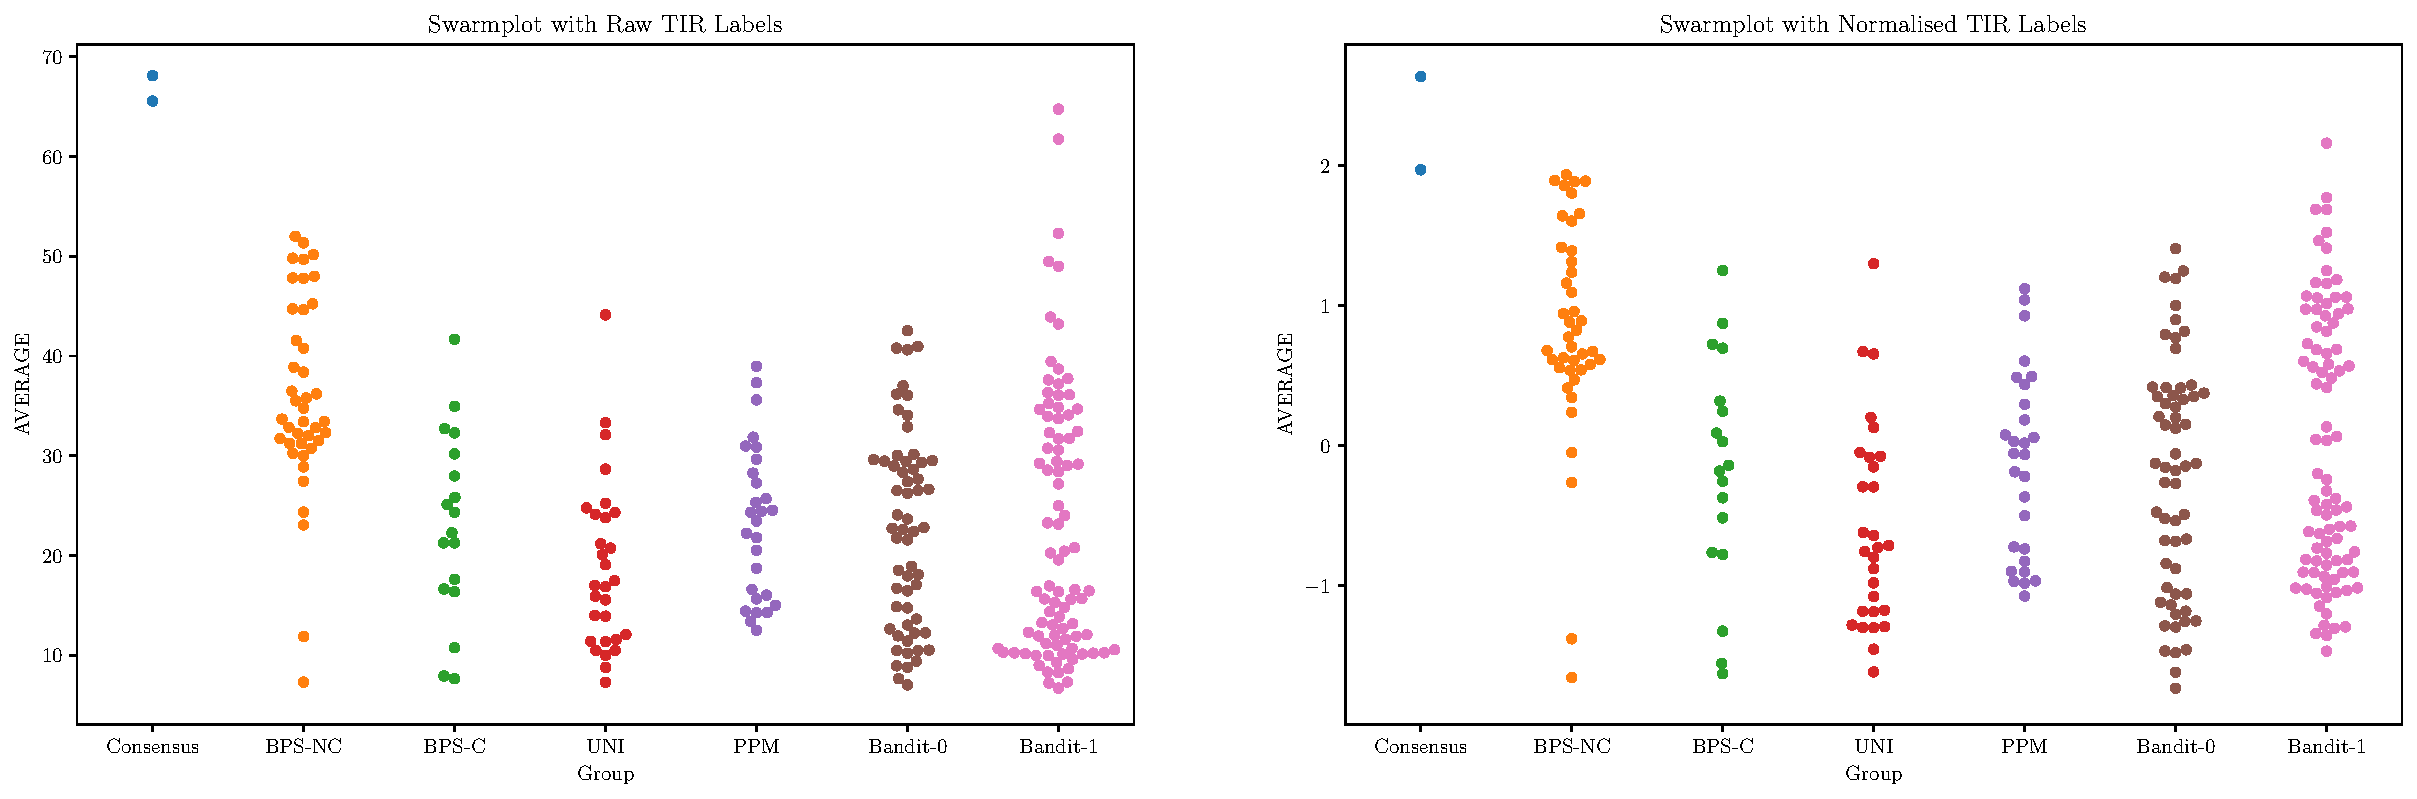
\includegraphics[scale = 0.4]{plots/Supplementary/swarmplots.pdf}
    \caption{Swarmplots for different groups, with raw (left) and normalised (right) TIR labels (averaged over 6 replicates). 
    Group names represent: Consensus (consensus sequence tested in different round); BPS-NC (bps noncore); BPS-C (bps core); UNI (uniformly random); PPM (position-based probability matrix); Bandit-0 (bandit design for round 0); Bandit-1 (bandit design for round 1).}
    \label{fig:swarmplots.}
\end{figure}

\begin{figure}
    \centering
    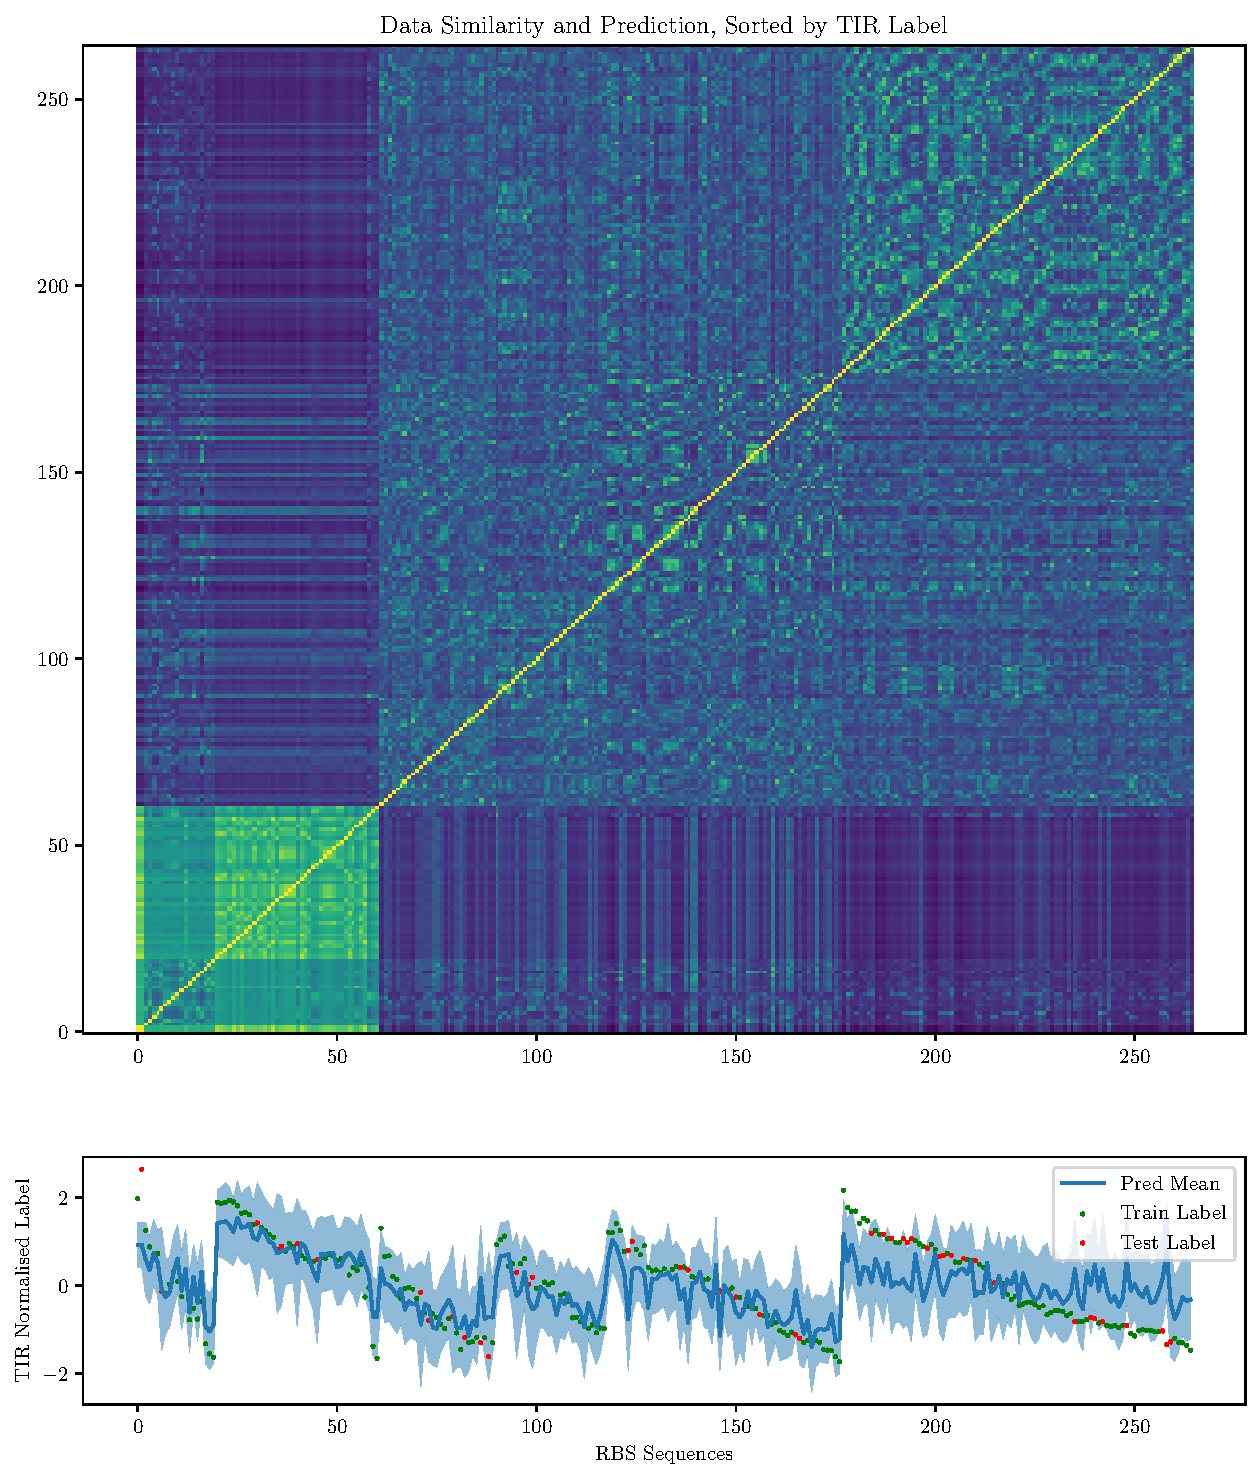
\includegraphics[scale = 0.3]{plots/Supplementary/Data_Similarity_and_Prediction_Sorted_by_TIR_Label.pdf}
    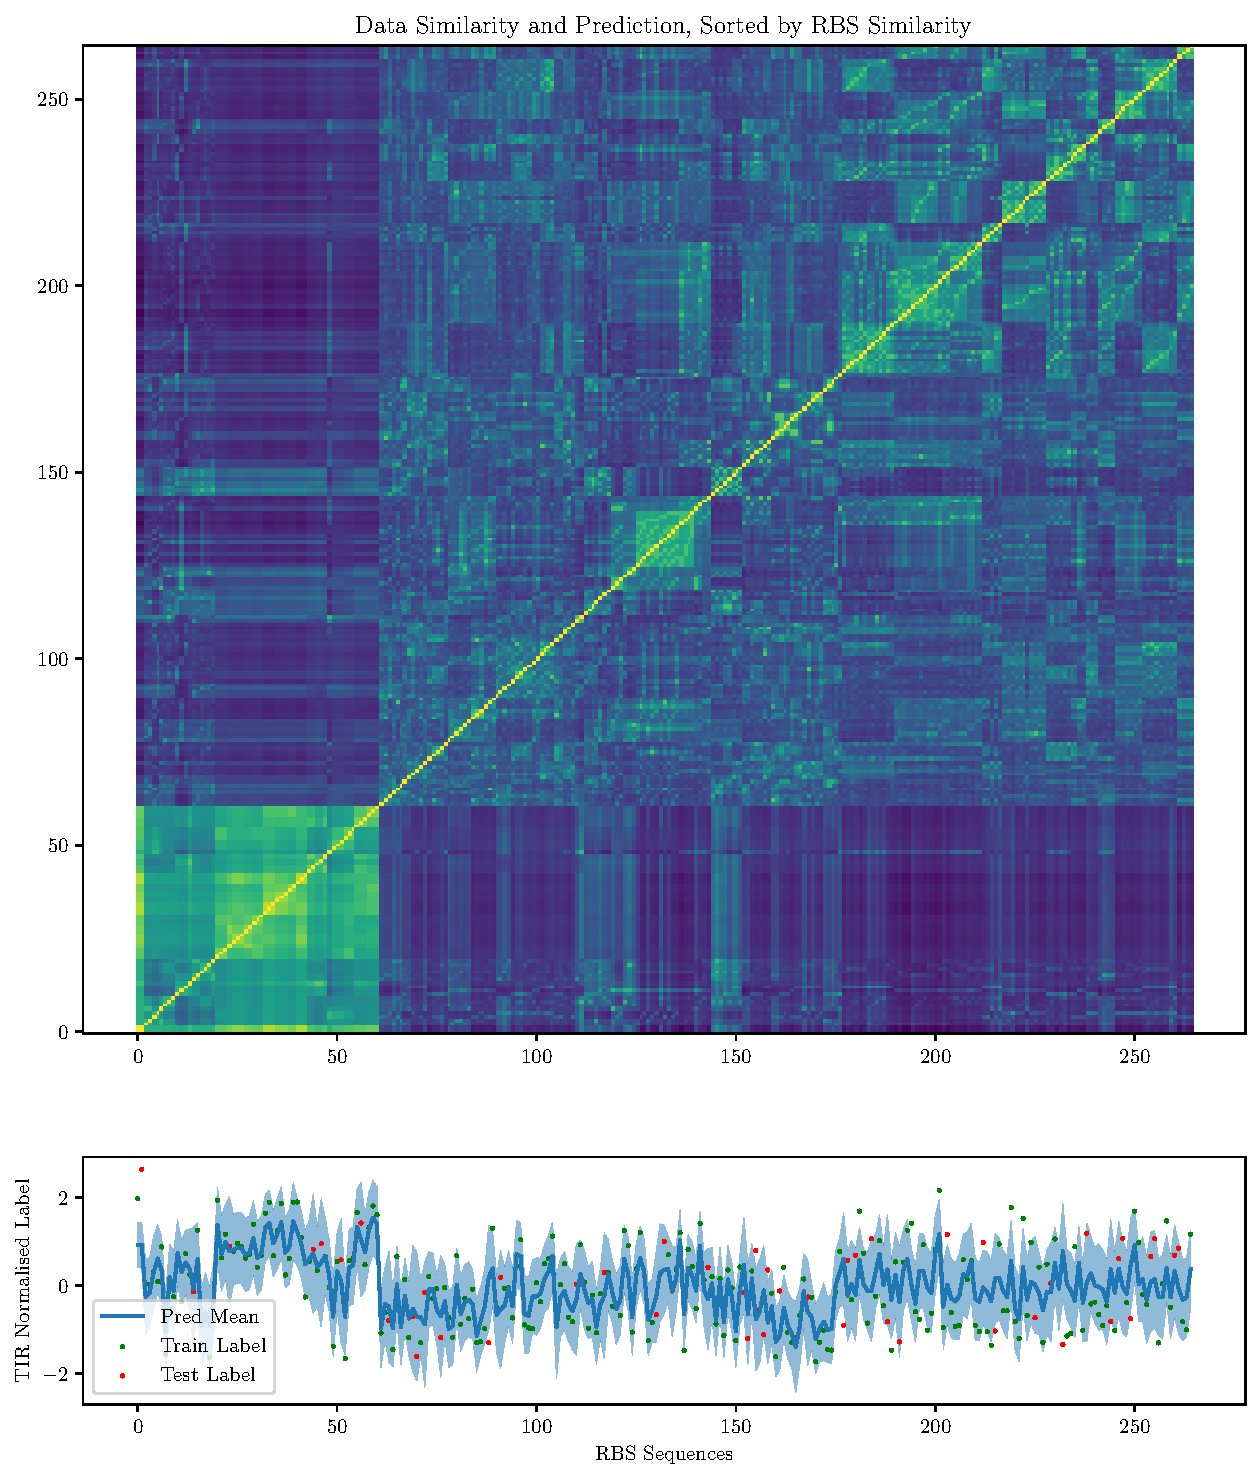
\includegraphics[scale = 0.3]{plots/Supplementary/Data_Similarity_and_Prediction_Sorted_by_RBS_Similarity.pdf}
    \caption{Kernel Heatmap and Predictions. Sequences are grouped as Consensus (1-2), BPS-C (3-20), BPS-NC (21-61), UNI (62-90), PPM (91-118), Bandit-0 (119-177), Bandit-1 (178-265). Inside of each group, sequences are clustered and sorted in terms of TIR labels (left) or RBS similarity (right). The first row shows the similarity measured by weighted degree kernel with shift, the second shows the predicted mean and uncertainty (1.95 standard deviation).}
    \label{fig:my_label}
\end{figure}

\begin{figure}
    \centering
    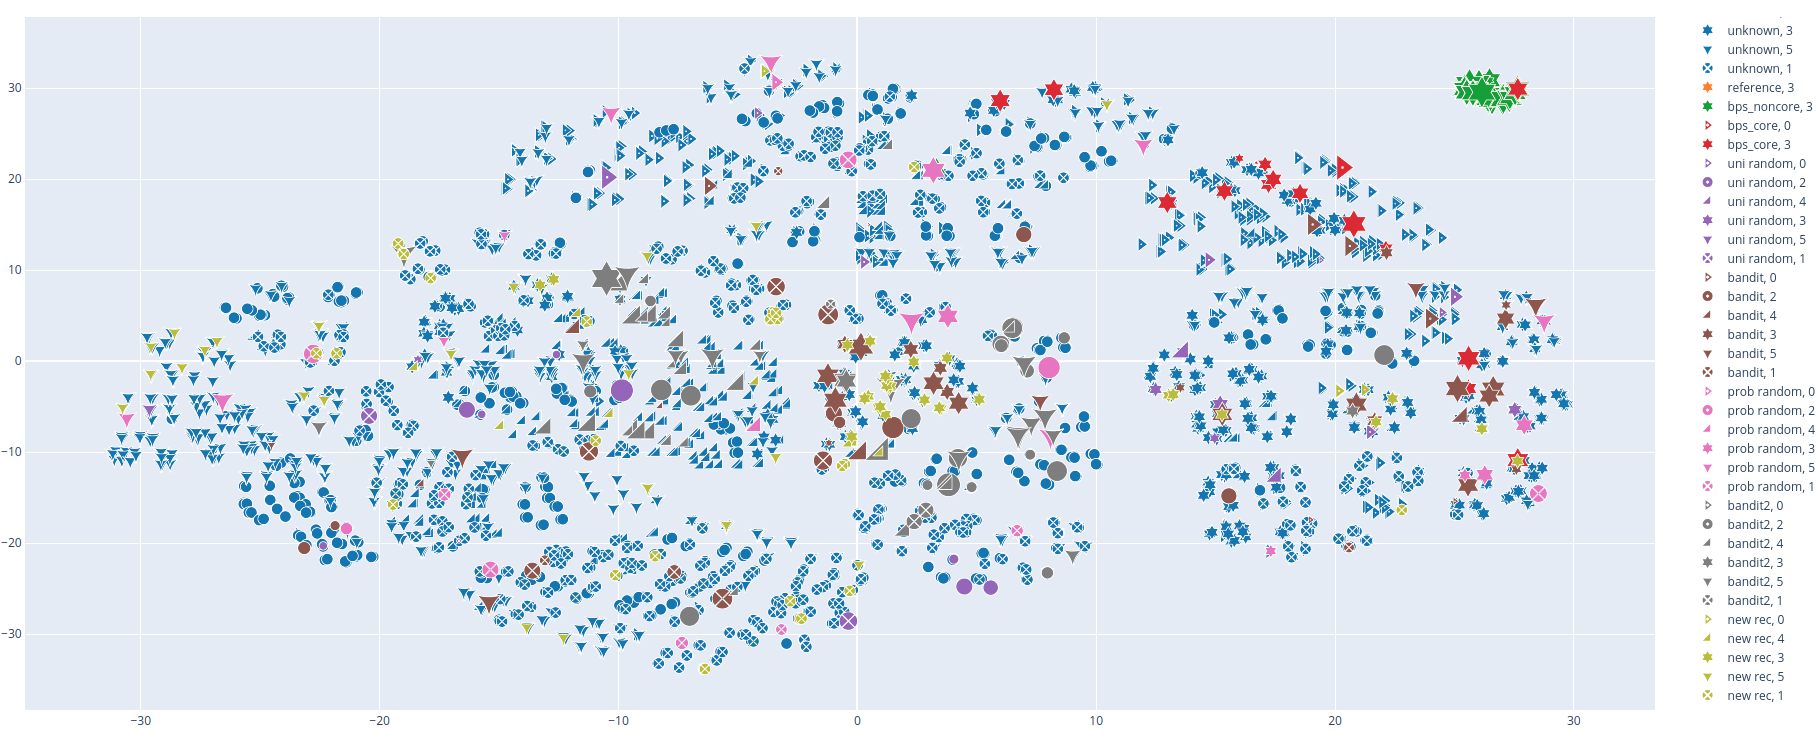
\includegraphics[scale = 0.25]{plots/Supplementary/clustering.png}
    \caption{TSNE of RBS sequences in design space with clustering. The distance is calculated based on the weighted degree kernel on RBS sequences. Colours indicate different groups, shapes indicate different clusters.}
    \label{fig:my_label}
\end{figure}

\subsection{Gaussian Process Regression}

A \textit{Gaussian process} is a collection of random variables, any finite number of which have a joint Gaussian distribution. 
We define mean function $\mu(\mathbf{x})$  and covariance function $k(\mathbf{x}, \mathbf{x}^\prime)$ of a real process $f(\mathbf{x})$ as
\begin{align}
    \mu(\mathbf{x}) &= \mathbb{E}[f(\mathbf{x})]\\
    k(\mathbf{x}, \mathbf{x}^\prime) &= \mathbb{E}[(f(\mathbf{x}) - \mu(\mathbf{x}))(f(\mathbf{x}^\prime) - \mu(\mathbf{x}^\prime))].
\end{align}

A Gaussian process is specified by its mean function and convariance function as $f(\mathbf{x}) \sim \mathcal{G} \mathcal{P}\left(\mu(\mathbf{x}), k\left(\mathbf{x}, \mathbf{x}^{\prime}\right)\right)$.
We consider the case where the observations are noisy, i.e. $\{(\mathbf{x}_i, y_i)| i = 1, \dots, n\}$, where $y_i = f(\mathbf{x}_i) + \epsilon$ with $\epsilon \sim \mathcal{N}(0, \alpha^2)$. 
The Gaussian noise is independent identically distributed, and the prior on the noisy observations is then $\operatorname{cov}\left(y_{p}, y_{q}\right)=k\left(\mathbf{x}_{p}, \mathbf{x}_{q}\right)+\alpha^{2} \delta_{p q}$,
where $\delta_{pq}$ is a Kronecker delta which is one if $p = q$ and zero otherwise.
It is equivalent to a diagonal matrix $\alpha^2 I$ on the kernel matrix evaluated on the training points.

For $n_\ast$ test points $X_\ast$, we assume the prior over the functions values as a random Gaussian vector $\mathbf{f}_\ast \sim \mathcal{N}(\mathbf{0}, K(X_\ast, X_\ast))$.
Then the joint distribution of the observed target values and the function values at the test points under the prior as 
\begin{align}
    \left[\begin{array}{l}\mathbf{y} \\ \mathbf{f}_{*}\end{array}\right] \sim \mathcal{N}\left(\mathbf{0},\left[\begin{array}{cc}K(X, X)+\alpha^{2} I & K\left(X, X_{*}\right) \\ K\left(X_{*}, X\right) & K\left(X_{*}, X_{*}\right)\end{array}\right]\right)
\end{align}
where $K(X, X_\ast)$ denotes the $n \times n_\ast$ covariance/Kernel matrix evaluated at all pairs of training and testing points, similarly for other kernel matrices.
Then the posterior of the test points (i.e. predictive distributions) is given by the conditional distribution $\mathbf{f}_\ast | X, \mathbf{y}, X_\ast \sim \mathcal{N}(\bar{\mathbf{f}}_\ast, cov(\mathbf{f}_\ast))$, where
\begin{align}
   \overline{\mathbf{f}}_{*} & \triangleq \mathbb{E}\left[\mathbf{f}_{*} \mid X, \mathbf{y}, X_{*}\right]=K\left(X_{*}, X\right)\left[K(X, X)+\alpha^{2} I\right]^{-1} \mathbf{y} \\
   \label{Eq: predicted variance}
   \operatorname{cov}\left(\mathbf{f}_{*}\right) &=K\left(X_{*}, X_{*}\right)-K\left(X_{*}, X\right)\left[K(X, X)+\alpha^{2} I\right]^{-1} K\left(X, X_{*}\right) 
\end{align}
For noisy test targets $\mathbf{y}_\ast$, we can compute the predictive distribution by adding $\alpha^2 I$ to the variance term $cov(\mathbf{f}_\ast)$ in Eq. (\ref{Eq: predicted variance}).
% We now introduce the marginal likelihood (or evidence) $p(\mathbf{y}|X)$, is which the integral of the likelihood times the prior 
% \begin{align}
%     p(\mathbf{y} \mid X)=\int p(\mathbf{y} \mid \mathbf{f}, X) p(\mathbf{f} \mid X) d \mathbf{f}
% \end{align}



\subsection{Choices of Kernels}

The choice of covariance function is critical for the performance of Gaussian process regression, we show a number of different string kernels tested in this study below:

\begin{itemize}
    \item \textit{Spectrum Kernel.}
    \begin{align}
        k_\ell^{\text{Spec}}(X, X^\prime) =\left\langle\phi_{\ell}^{\mathrm{Spec}}(\mathbf{x}), \phi_{\ell}^{\mathrm{Spec}}\left(\mathbf{x}^{\prime}\right)\right\rangle = \phi_{\ell}^{\mathrm{Spec}}(\mathbf{x})^T \phi_{\ell}^{\mathrm{Spec}}\left(\mathbf{x}^{\prime}\right).
    \end{align}
     where $\mathbf{x}, \mathbf{x}^\prime$ are two RBS sequences in $\mathcal{D}$ over an alphabet $\Sigma$. We denote the number of letters in the alphabet as $|\Sigma|$. 
    $\phi_{\ell}^{\mathrm{spec}}(\mathbf{x})$ maps the sequence $X$ into a $|\Sigma|^\ell$ dimensional feature space, where each dimension is the count of the number of one of the $|\Sigma|^\ell$ possible strings $s$ of length $\ell$. 
    Let $X, X^\prime$ be two metrics which include $n$ sequences, and $\Phi_d^{Spec}(X) \in \mathbb{R}^{n \times |\Sigma|^{\ell}}$, then the spectrum kernel over metrics is 
    \begin{align}
         K_\ell^{\text{Spec}}(X, X^\prime) = \Phi_{\ell}^{\mathrm{Spec}}(X) \Phi_{\ell}^{\mathrm{Spec}}\left(X^{\prime}\right)^T.
    \end{align}
    
    \item \textit{Sum of Spectrum Kernel,} considers weighted sum over different parts of the string. 
    
    \item \textit{Mixed Spectrum Kernel,} considers weighted sum over different substring length, with $\beta_d = \frac{2(\ell - d + 1)}{\ell(\ell+1)}$,
        \begin{align}
            k_\ell^{MixedSpec}(\mathbf{x}, \mathbf{x}^\prime) 
            = \sum_{d=1}^{\ell} \beta_d k_d^{Spec}(\mathbf{x}, \mathbf{x}^\prime)
        \end{align}
    \item \textit{Weighted Degree Kernel,} considers positional information. WD kernel counts the match of kmers at corresponding positions in two sequences.
    For sequences with fixed length $L$ and weighted degree kernel considers substrings starting at each position $l = 1, ..., L$, with $\beta_d = \frac{2(\ell - d + 1)}{\ell(\ell+1)}$, \\
    \begin{align}
        k_\ell^{WD}(\mathbf{x}, \mathbf{x}^\prime) 
        &= \sum_{d=1}^{\ell} \beta_d \sum_{l=1}^{L-d+1} \gamma_l k_d^{Spec}(\mathbf{x}_{[l:l+d]}, \mathbf{x}_{[l:l+d]}^\prime)\\
        &= \sum_{d=1}^{\ell} \beta_d \sum_{l=1}^{L-d+1} \gamma_l \phi_d^{Spec}(\mathbf{x}_{[l:l+d]})^T \phi_d^{Spec}(\mathbf{x}_{[l:l+d]}^\prime)\\
        &= \sum_{d=1}^{\ell} \beta_d \sum_{l=1}^{L-d+1} \gamma_l \mathbb{I}(\mathbf{x}_{[l:l+d]} = \mathbf{x}_{[l:l+d]}^\prime),
    \end{align}
    where $\mathbb{I}(\text{true}) = 1$ and 0 otherwise. 
    
    \item \textit{Weighted Degree Kernel With Shift.}
    \begin{align}
        k_\ell^{WDS}(\mathbf{x}, \mathbf{x}^\prime) 
        &= \sum_{d=1}^{\ell} \beta_d \sum_{l=1}^{L-d+1} \gamma_l \sum_{s = 0, s + l \leq L}^{S(l)} \delta_s
        \left(k_d^{Spec}(\mathbf{x}_{[l+s:l+s+d]}, \mathbf{x}_{[l:l+d]}^\prime) + (k_d^{Spec}(\mathbf{x}_{[l:l+d]}, \mathbf{x}_{[l+s:l+s+d]}^\prime)\right)\\
        &= \sum_{d=1}^{\ell} \beta_d \sum_{l=1}^{L-d+1} \gamma_l \sum_{s = 0, s + l \leq L}^{S(l)} \delta_s
        \left(\mathbb{I}(\mathbf{x}_{[l+s:l+s+d]} = \mathbf{x}_{[l:l+d]}^\prime) + (\mathbb{I}(\mathbf{x}_{[l:l+d]}= \mathbf{x}_{[l+s:l+s+d]}^\prime)\right),
    \end{align}
    where $\beta_d = \frac{2(\ell - d + 1)}{\ell(\ell+1)}, \delta_s = \frac{1}{2(s+1)}$, $\gamma_l$ is a weighting over the position in the
    sequence, where we choose to use a uniform weighting over the sequences, i.e. $\gamma_l = 1/L$. $S(l)$ determines the shift
    range at position $l$.
\end{itemize}

\textbf{From kernel to distance}:
$$d(\mathbf{x}, \mathbf{x}^\prime) = \sqrt{k(\mathbf{x}, \mathbf{x}) + k(\mathbf{x}^\prime, \mathbf{x}^\prime) - 2 k(\mathbf{x}, \mathbf{x}^\prime)} $$

\subsubsection{Normalisation of Kernel}

As part of data pre-processing,
the range of all features should be normalised so that each feature contributes approximately proportionately to the predictive model. 
The kernel matrix is represented by the inner product of the underlying feature vectors, it needs to be normalised before being used in the downstream regression models. 
Up-scaling (down-scaling) features can be understood as down-scaling (up-scaling) regularizers such that they penalise the features less (more). 

Here we consider two approaches for kernel normalisation: centering and unit norm. 
We will show how to convert the normalisation in terms of feature vectors to normalisation in terms of kernel matrices. 
As defined before, consider $\mathbf{x}, \mathbf{x}^\prime$ are two RBS sequences in $\mathcal{D}$ over an alphabet $\Sigma$.
We denote $\phi(\mathbf{x}_i)$ as a column feature vector of sequence $\mathbf{x}_i$, 
where a feature function $\phi: \mathbf{x} \rightarrow \mathbb{R}^d$. Assume there is total of $n$ sequences in the data $X$ ($n'$ sequences in the data $X'$). 
We illustrate centering and unit norm normalisation below. 

\begin{itemize}
    \item Centering. 
    Defining the mean vector as $\bar{\Phi}(X) = \frac{1}{n} \sum_{s = 1}^n \phi(\mathbf{x}_s) \in \mathbb{R}^d$, the centered feature vector $\phi^C(\mathbf{x}_i) \in \mathbb{R}^d$ of $\mathbf{x}_i$ is
    \begin{align}
        \phi^{C}(\mathbf{x}_i) = \phi(\mathbf{x}_i) - \bar{\Phi}(X) = \phi(\mathbf{x}_i) - \frac{1}{n'} \sum_{s = 1}^{n'} \phi(\mathbf{x}_s).
    \end{align}
    The corresponding centering kernel value between $\mathbf{x}_i$ and $\mathbf{x}_j$ is then 
    \begin{align}
        k^C(\mathbf{x}_i, \mathbf{x}_j) &= <\phi^C(\mathbf{x}_i), \phi^C(\mathbf{x}_j)>\\
        &= \left( \phi(\mathbf{x}_i) - \frac{1}{n} \sum_{s = 1}^n \phi(\mathbf{x}_s)\right)^T \left( \phi(\mathbf{x}_j) - \frac{1}{n'} \sum_{s' = 1}^{n'} \phi(\mathbf{x}_{s'})\right)\\
        &= \phi(\mathbf{x}_i)^T \phi(\mathbf{x}_j) - \left( \frac{1}{n} \sum_{s = 1}^n \phi(\mathbf{x}_s)\right)^T \phi(\mathbf{x}_j) - \phi(\mathbf{x}_i)^T \left(\frac{1}{n} \sum_{s' = 1}^{n'} \phi(\mathbf{x}_{s'})\right) + \left( \frac{1}{n} \sum_{s = 1}^n \phi(\mathbf{x}_s)\right)^T \left(\frac{1}{n'} \sum_{s' = 1}^{n'} \phi(\mathbf{x}_{s'})\right)\\
        &= k(\mathbf{x}_i, \mathbf{x}_j) - \frac{1}{n} \sum_{s=1}^n k(\mathbf{x}_s, \mathbf{x}_j) - \frac{1}{n'} \sum_{s'=1}^{n'} k(\mathbf{x}_i, \mathbf{x}_{s'}) + \frac{1}{n^2} \sum_{s = 1}^n \sum_{s'=1}^{n'} k(\mathbf{x}_s, \mathbf{x}_{s'})
    \end{align}
    
    \item Unit Norm. Define the ($l_2$) norm of a feature vector as $||\phi(\mathbf{x})|| = \sqrt{\sum_{m = 1}^d \phi_d(\mathbf{x})^2} = \sqrt{k(\mathbf{x}, \mathbf{x})} \in \mathbb{R}^+$, then the unit norm feature vector $\phi^{UN}(\mathbf{x}_i) \in \mathbb{R}^d$ of $\mathbf{x}_i$ is 
    \begin{align}
        \phi^{UN}(\mathbf{x}_i) = \frac{\phi(\mathbf{x}_i)}{||\phi(\mathbf{x}_i)||}.
    \end{align}
    The corresponding unit norm kernel value between $\mathbf{x}_i$ and $\mathbf{x}_j$ is then 
    \begin{align}
        k^{UN}(\mathbf{x}_i, \mathbf{x}_j) &= <\frac{\phi(\mathbf{x}_i)}{||\phi(\mathbf{x}_i)||}, \frac{\phi(\mathbf{x}_j)}{||\phi(\mathbf{x}_j)||}>\\
        &= \frac{\phi(\mathbf{x}_i)^T \phi(\mathbf{x}_j)}{||\phi(\mathbf{x}_i)|| \times ||\phi(\mathbf{x}_j)||}\\
        &= \frac{k(\mathbf{x}_i, \mathbf{x}_j)}{\sqrt{k(\mathbf{x}_i, \mathbf{x}_i)  k(\mathbf{x}_j, \mathbf{x}_j)}}
    \end{align}
    
     \item Unit Variance. 
    After the centering and unit norm normalisation, the kernel matrix is unit variance as well. 
    In the following, we show transformations of the unit variance (with centering) normalisation.
    Define the variance vector ${Var}(\Phi(X)) = \frac{1}{n} \sum_{s=1}^n ||\phi(\mathbf{x}_s) - \bar{\Phi}(X)||^2 = \frac{1}{n} \sum_{s=1}^n ||\phi(\mathbf{x}_s) - \sum_{s'=1}^n \left(\phi(\mathbf{x}_s')\right)||^2 = \frac{1}{n} \sum_{s=1}^n  k^C(\mathbf{x}_s, \mathbf{x}_s)  \in \mathbb{R}$, the unit variance feature vector $\phi^{UV}(\mathbf{x}_i) \in \mathbb{R}^d$ of $\mathbf{x}_i$ is
    \begin{align}
        \phi^{UV}(\mathbf{x}_i) = \frac{\phi(\mathbf{x}_i)}{\sqrt{Var(\Phi(X))}}.
    \end{align}
    The corresponding kernel representation is 
    \begin{align}
        k^{UV}(\mathbf{x}_i, \mathbf{x}_j) &= <\frac{\phi(\mathbf{x}_i)}{\sqrt{Var(\Phi(X))}}, \frac{\phi(\mathbf{x}_j)}{\sqrt{Var(\Phi(X'))}}>\\
        &= \frac{\phi(\mathbf{x}_i)^T \mathbf{x}_j}{\sqrt{Var(\Phi(X)) Var(\Phi(\mathbf{X'}))}}\\
        &= \frac{k(\mathbf{x}_i, \mathbf{x}_j)}{\sqrt{ \frac{1}{n} \sum_{s=1}^n  k^C(\mathbf{x}_s, \mathbf{x}_s)  \frac{1}{n} \sum_{s'=1}^{n'}  k^C(\mathbf{x}_{s'}, \mathbf{x}_{s'})}}
    \end{align}
    After centering and unit norm, $ \frac{1}{n} \sum_{s=1}^n  k^C(\mathbf{x}_s, \mathbf{x}_s) = k(\mathbf{x}_i, \mathbf{x}_i)$, which implies that after centering and unit norm, the kernel matrix is already unit variance normalised. 
\end{itemize}
For the Gaussian Process regression, we make of use of two kernel matrices: the kernel function between the training data itself, i.e. $K(X_{train}, X_{train})$; and
the kernel function taking the training data and testing data as inputs, i.e. $K(X_{test}, X_{train})$. 
%It is straightforward to normalise a square kernel which same input, i.e. $n = n'$ and $k(\mathbf{x}_i, \mathbf{x}_i),  k(\mathbf{x}_j, \mathbf{x}_j)$ taken from the diagonal of the matrix. 
%The second one (between train and test) is a little bit tricky. The different is not only that $n \neq n'$. 
We will state two ways of normalisation those two kind of matrices:
\begin{itemize}
    \item Normalise training and testing data separately.
    This approach is preferred for most of the machine learning algorithms since it follows the rule that we have no information about testing data while training.
    Then for centering, one should subtract the mean vector over the training data for both kinds of matrices.
    For unit norm normalisation, when one calculates $K^{UN}(X_{test}, X_{train})$, the two terms inside of square root: $k(\mathbf{x}_i, \mathbf{x}_i)$ is taken from $K(X_{test}, X_{test})[i,i]$, and $k(\mathbf{x}_j, \mathbf{x}_j)$ is taken from $K(X_{train}, X_{train})[j,j]$.
    
    \item Normalise training and testing data together, i.e. normalise $K(X_{train+test}, X_{train+test})$, then extra the parts we need from the normalised matrix. 
    This approach is suitable in a case where one already knows the whole of testing features. 
    For centering, one should subtract the mean vector over the whole matrix $\Phi(X_{train+test})$. 
    The unit norm normalisation is the same as in the previous case. 
\end{itemize}

For our experiment, we fix the design space before training, i.e. the testing features are already known before testing. 
So we choose to normalise the kernel matrix over the training and testing data together,
by first applying centering and then unit norm normalisation. 

\subsection{Batch Recommendation}

For recommending RBS sequences to label, we consider the Upper Confidence Bound (UCB) algorithm, 
%which is based on the \textit{optimism in the face of uncertainty}, 
selecting RBS sequences with the maximum upper confidence bound at round $t$, i.e.
\begin{align}
\label{Eq: GPUCB}
    \operatorname{argmax}_{\mathbf{x}_i \in \mathcal{D}} \left( \mu_{t-1}(\mathbf{x}_i) + \beta_t \sigma_{t-1}(\mathbf{x}_i)\right),
\end{align}
where $\beta_t$ is a hyperparmeter balancing the exploitation and exploration, 
$\mu_t(\mathbf{x}_i), \sigma_t(\mathbf{x}_i)$ are the predicted mean and standard deviation at round $t$ for the sequence $\mathbf{x}_i$.

Since labelling sequences is time-consuming, it is unrealistic to recommend sequence sequentially (i.e. one-by-one) and waiting for the label after each prediction.
Therefore we consider recommending sequences in batch and using Gaussian Process Batch Upper Confidence Bound (GP-BUCB) algorithm  \cite{desautels2012parallelizing}.
With batches of size $B$, the feedback mapping $fb[t] = \lfloor(t-1) / B\rfloor B$, i.e. 
\begin{align}
    \mathrm{fb}[t]=\left\{\begin{array}{cl}
    0 & : t \in\{1, \ldots, B\} \\
    B & : t \in\{B+1, \ldots, 2 B\} \\
    2 B & : t \in\{2 B+1, \ldots, 3 B\} \\
    & \vdots
    \end{array}\right.
\end{align}


A key property of Gaussian Process regression is that the predictive variance in Eq. (\ref{Eq: predicted variance}) only depends on observed points (i.e. features), but not on the labels of these observed points. 
So one can compute the posterior variance without actually observing the labels. 
The GP-BUCB policy is to select sequences that
\begin{align}
    \operatorname{argmax}_{\mathbf{x}_i \in \mathcal{D}} \left( \mu_{fb[t]}(\mathbf{x}_i) + \beta_t \sigma_{t-1}(\mathbf{x}_i)\right).
\end{align}
And only update $y_{t^{\prime}}=f\left(\boldsymbol{x}_{t^{\prime}}\right)+\varepsilon_{t^{\prime}} \text { for } t^{\prime} \in\{\mathrm{fb}[t]+1, \ldots, \mathrm{fb}[t+1]\}$ at the end of each batch ($\mathrm{fb}[t]<\mathrm{fb}[t+1]$). 
This is equivalent to sequential GP-UCB with \textit{hallucinated observations} $\boldsymbol{y}_{\mathrm{fb}[t]+1: t-1}=\left[\mu_{\mathrm{fb}[t]}\left(\boldsymbol{x}_{\mathrm{fb}[t]+1}\right), \ldots, \mu_{\mathrm{fb}[t]}\left(\boldsymbol{x}_{t-1}\right)\right]$, while the posterior variance decreases. 


\subsection{Design Pipeline}

The n + 1 round design is based on the nth round result, where each sequence has 6 replicates with TIR labels.
We pre-processed the data by taking a logarithm transformation and standardisation of the raw TIR label for each replicates respectively, where TIR is calculated as a derivative of GFP fluoresence divided by OD600 of culture over 4h counting from the start of log phase of growth. 
After normalisation, each replicate has zero mean and unit variance. 

For prediction, we use Gaussian process regression, with training on all normalised replicates and predicting on the design space (6-base core part design) except known sequences. 
We assume the observation are noisy, where the noise is under centered normal distribution with standard deviation $\alpha$.  
We model the covariance matrix using the weighted degree kernel with shift. 
We normalise the kernel with centering and unit norm in terms of the whole kernel constructed by both first round result and design space. 
The hyperparameter for kernel, including maximum substring length  $l$, maximum shift length $s$, and the noise standard deviation $\alpha$ of Gaussian process model are choose based on 10-repeat 5-fold cross validation. 
We choose $l=6, s= 1, \alpha = 2$ for the second round design. 

For recommendation, we use batch upper confidence bound introduced by GP-BUCB algorithm \cite{desautels2012parallelizing}. 
The upper confidence bound is constructed by predicted mean plus 2 predicted standard deviation.   
We recommend 90 sequences from the design space. 



\subsection{Intuition behind UCB and visualisation}

\begin{itemize}
    \item Exploitation and exploration explanation.
    \item Visualise coverage by clustering plot.
    \item Table for in-clustering mean and variance.
\end{itemize}

\subsection{Result analysis}

\begin{itemize}
    \item violinplot.
    \item regression performance plot, table.
    \item kernel matrix plot.
\end{itemize}

\subsection{Statistics of the core vs non-core regions of the RBS}

In our study, we have tested a set of sequnces designed to confirm the notion that changing bases within the RBS core (6 bases) is statistically more influencing the TIR than the changes made outside the core.
This hypothesis has been build based on reported biases towards certain bases present in the core of the RBS but absent outside of it.
For example, according to \cite{SHULTZABERGER2001} there is a strong bias towards A and G bases in the core region of the RBS.
Similarly outside of the 6 bases of the core in the wider 20 bp context of the RBS there is no significant bias towards any particular base which suggest that these bases do not contribute to the overal TIR of a given RBS. 
This effect is shown in (Figure \ref{fig:core_vs_noncore}), which shows results for our set X of sequences.
The value of Welch's t-test between the mean TIR in core and non-core groups is -4.8780 with p-value < 0.0001 and 34 degrees of Freedom.

\begin{figure}[h]
    \centering
    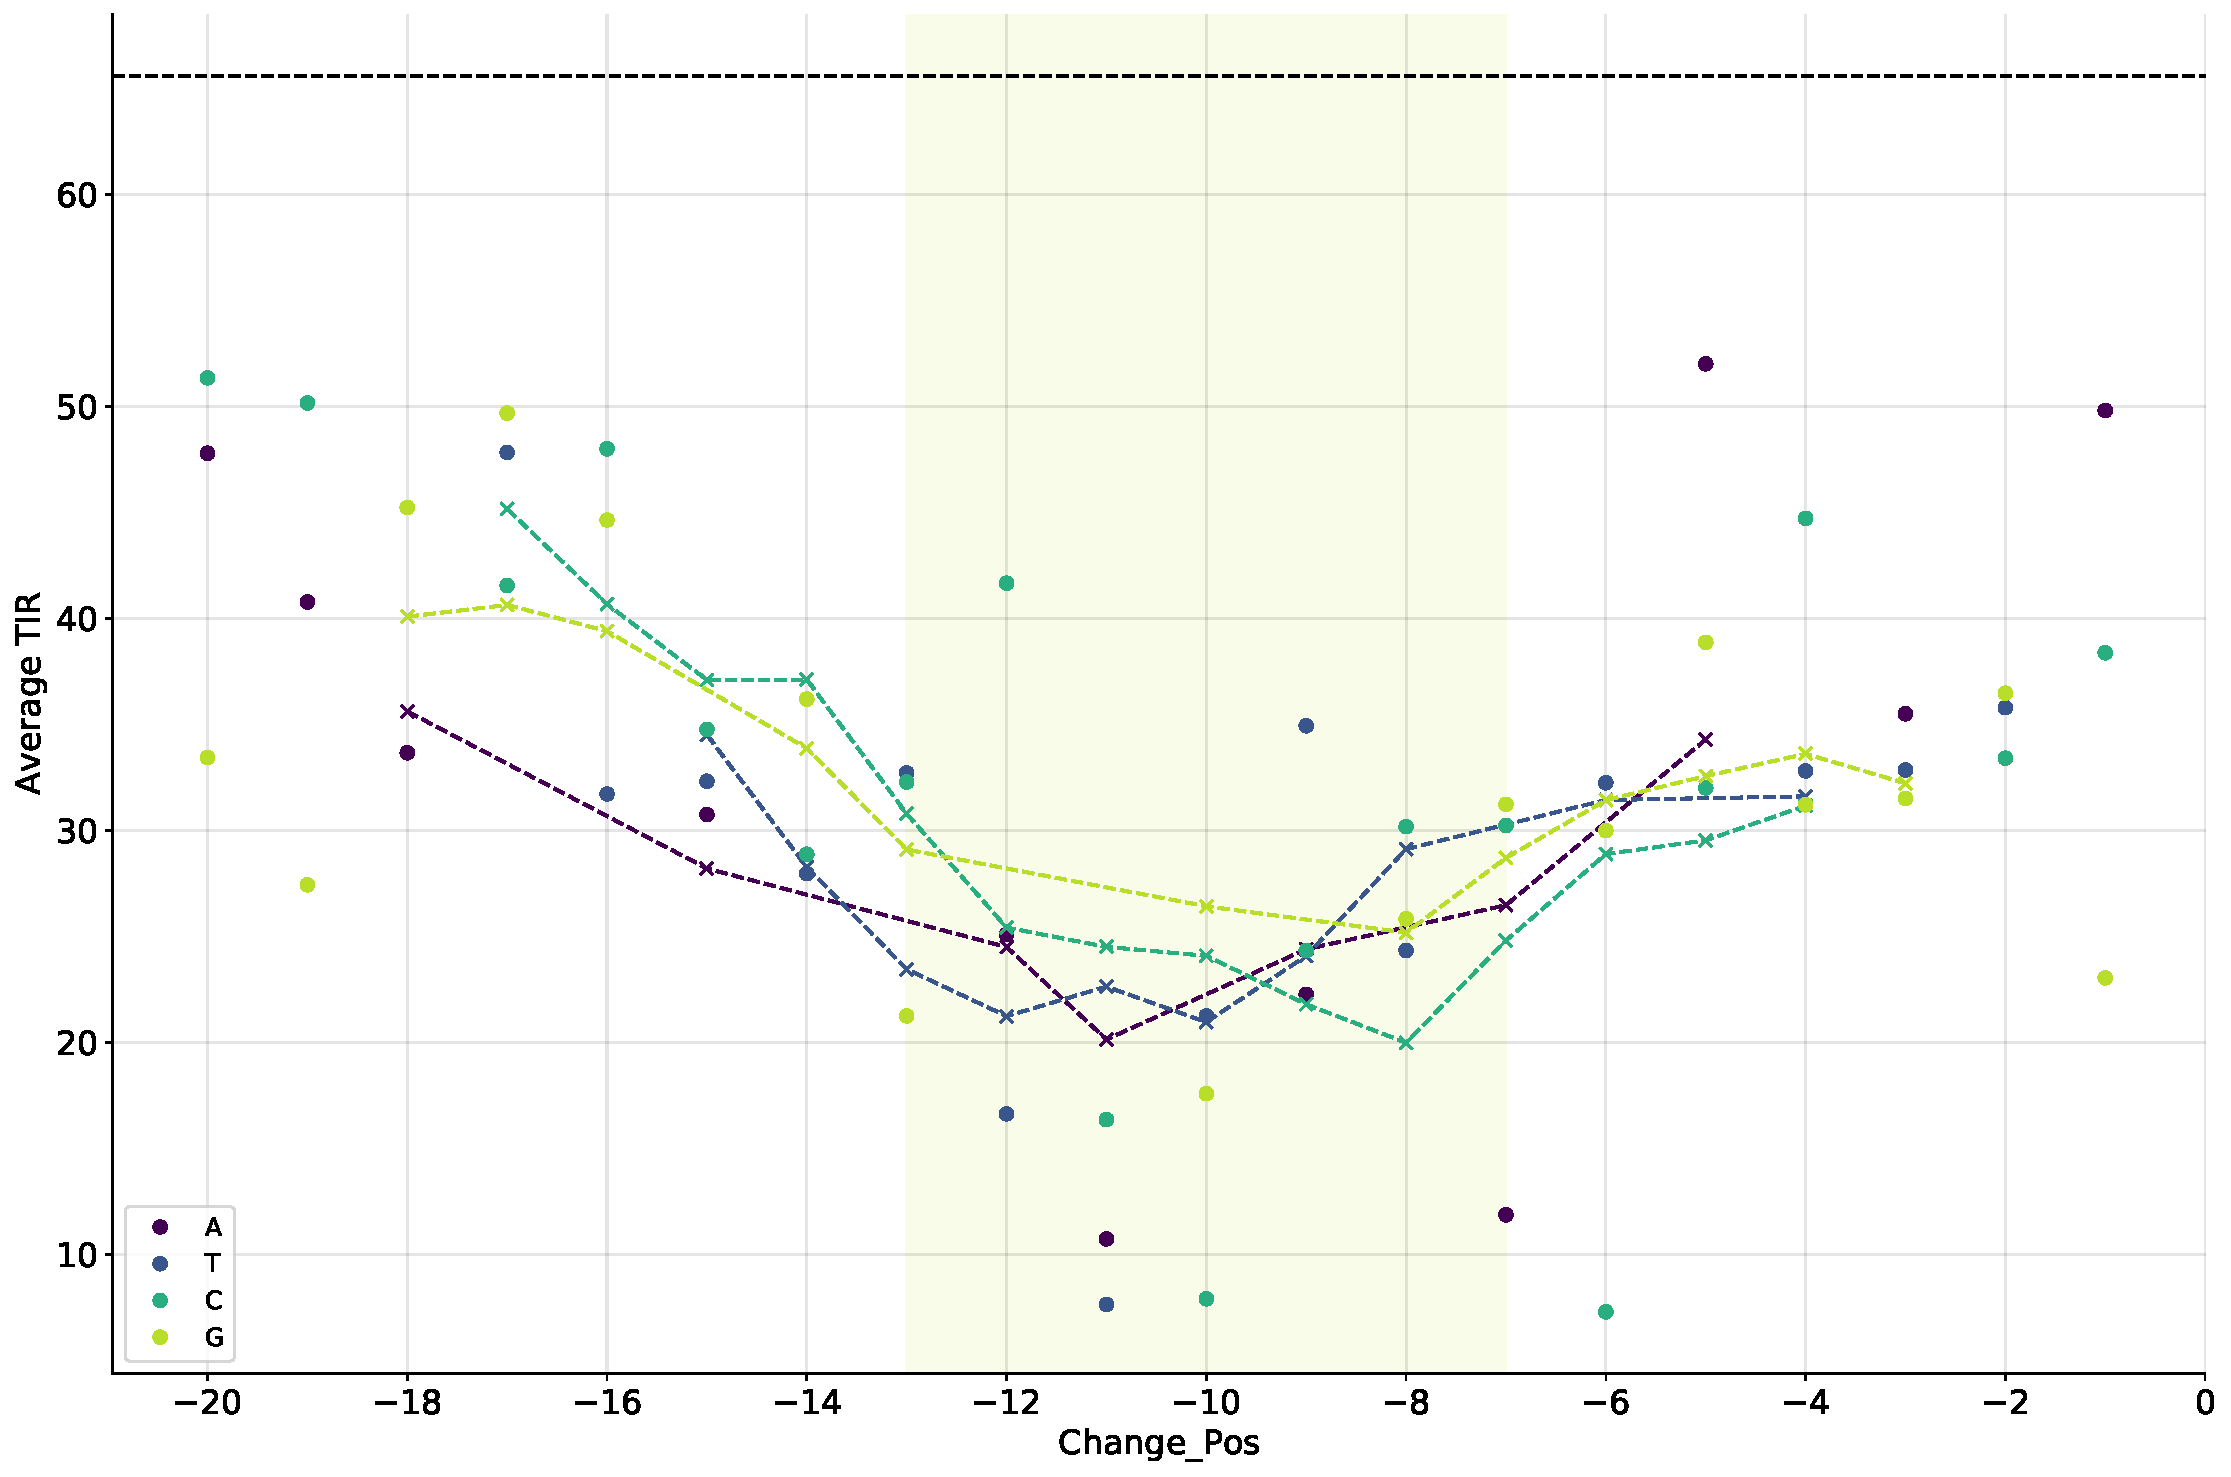
\includegraphics[scale=0.4]{plots/Supplementary/core_vs_noncore.pdf}
    \caption{\textbf{Comparison of base change impact on TIR in core versus non-core region.} The core region is highligthed in light green and the lines are rolling averages for each base. The top dotted line shows the TIR for the benchmark sequence, where dots represent a change at a given position to a given base, which is colour coded.}
    \label{fig:core_vs_noncore}
\end{figure}

\section{Supplementary Figures}

\begin{figure}
     \centering
     \begin{subfigure}[b]{0.49\textwidth}
         \centering
         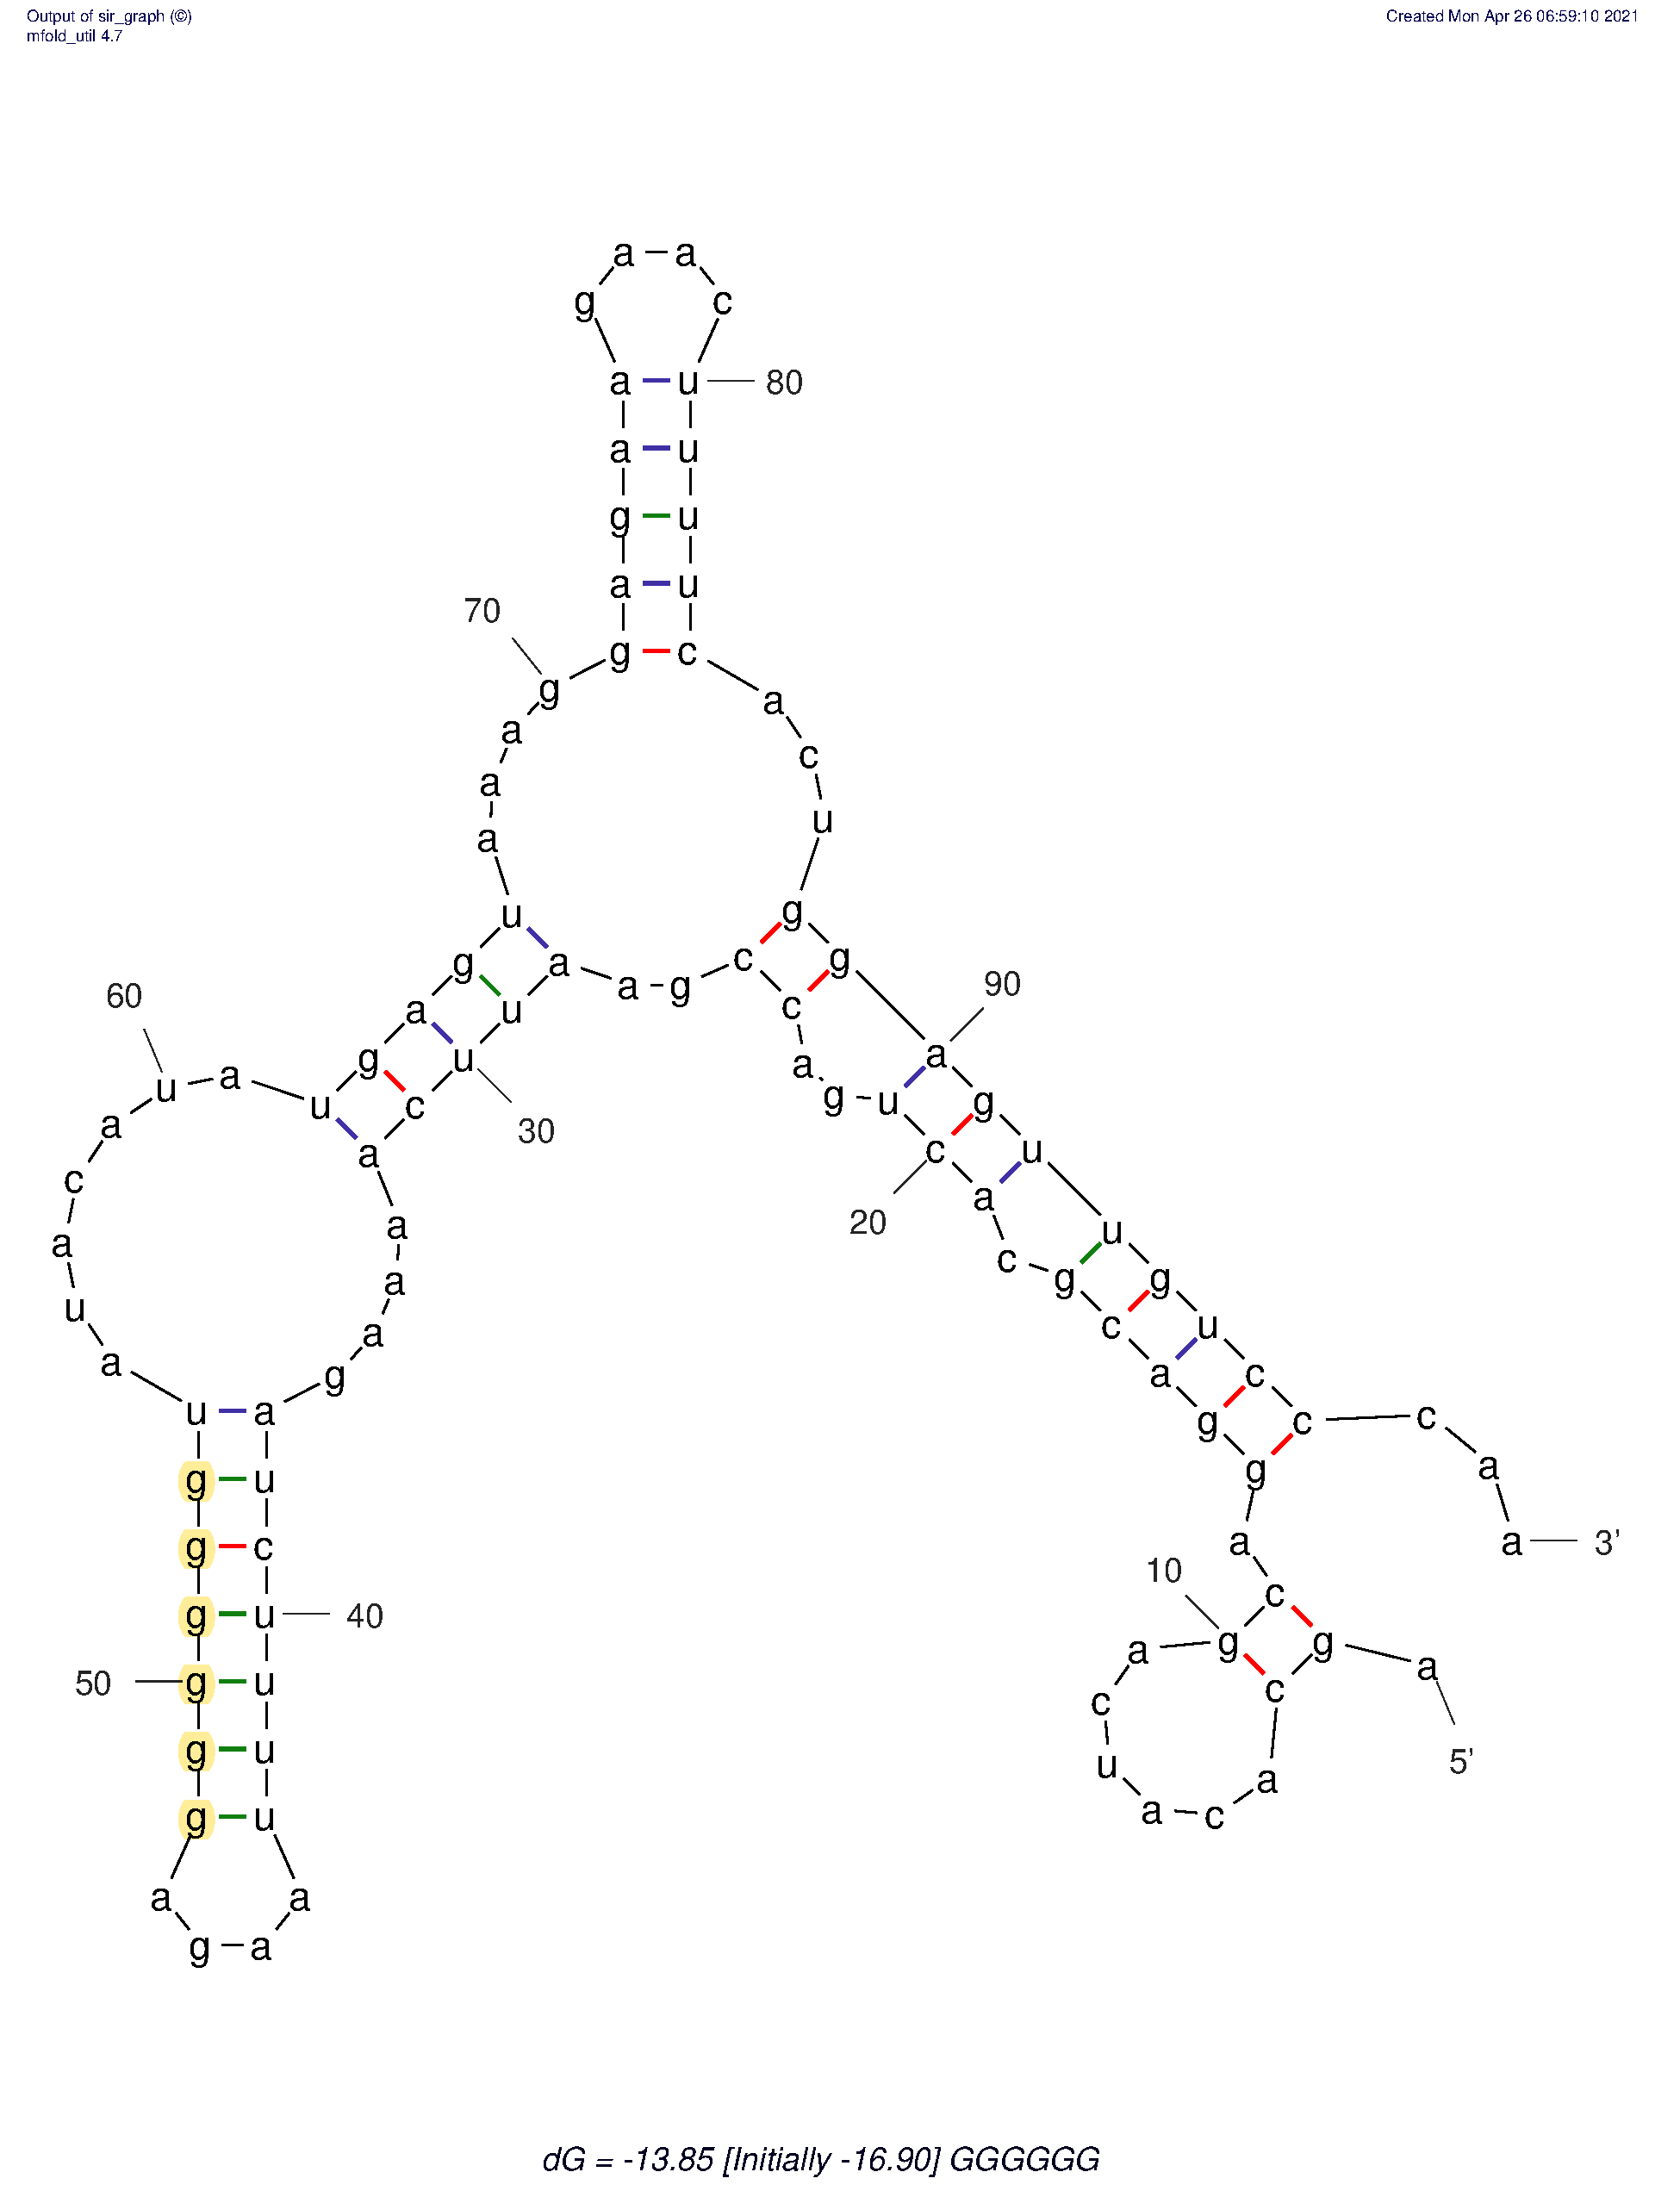
\includegraphics[scale=0.25]{plots/Supplementary/Structure GGGGGG.pdf}
         \caption{$y=x$}
         \label{fig:GGGGGG}
     \end{subfigure}
     \hfill
     \begin{subfigure}[b]{0.49\textwidth}
         \centering
         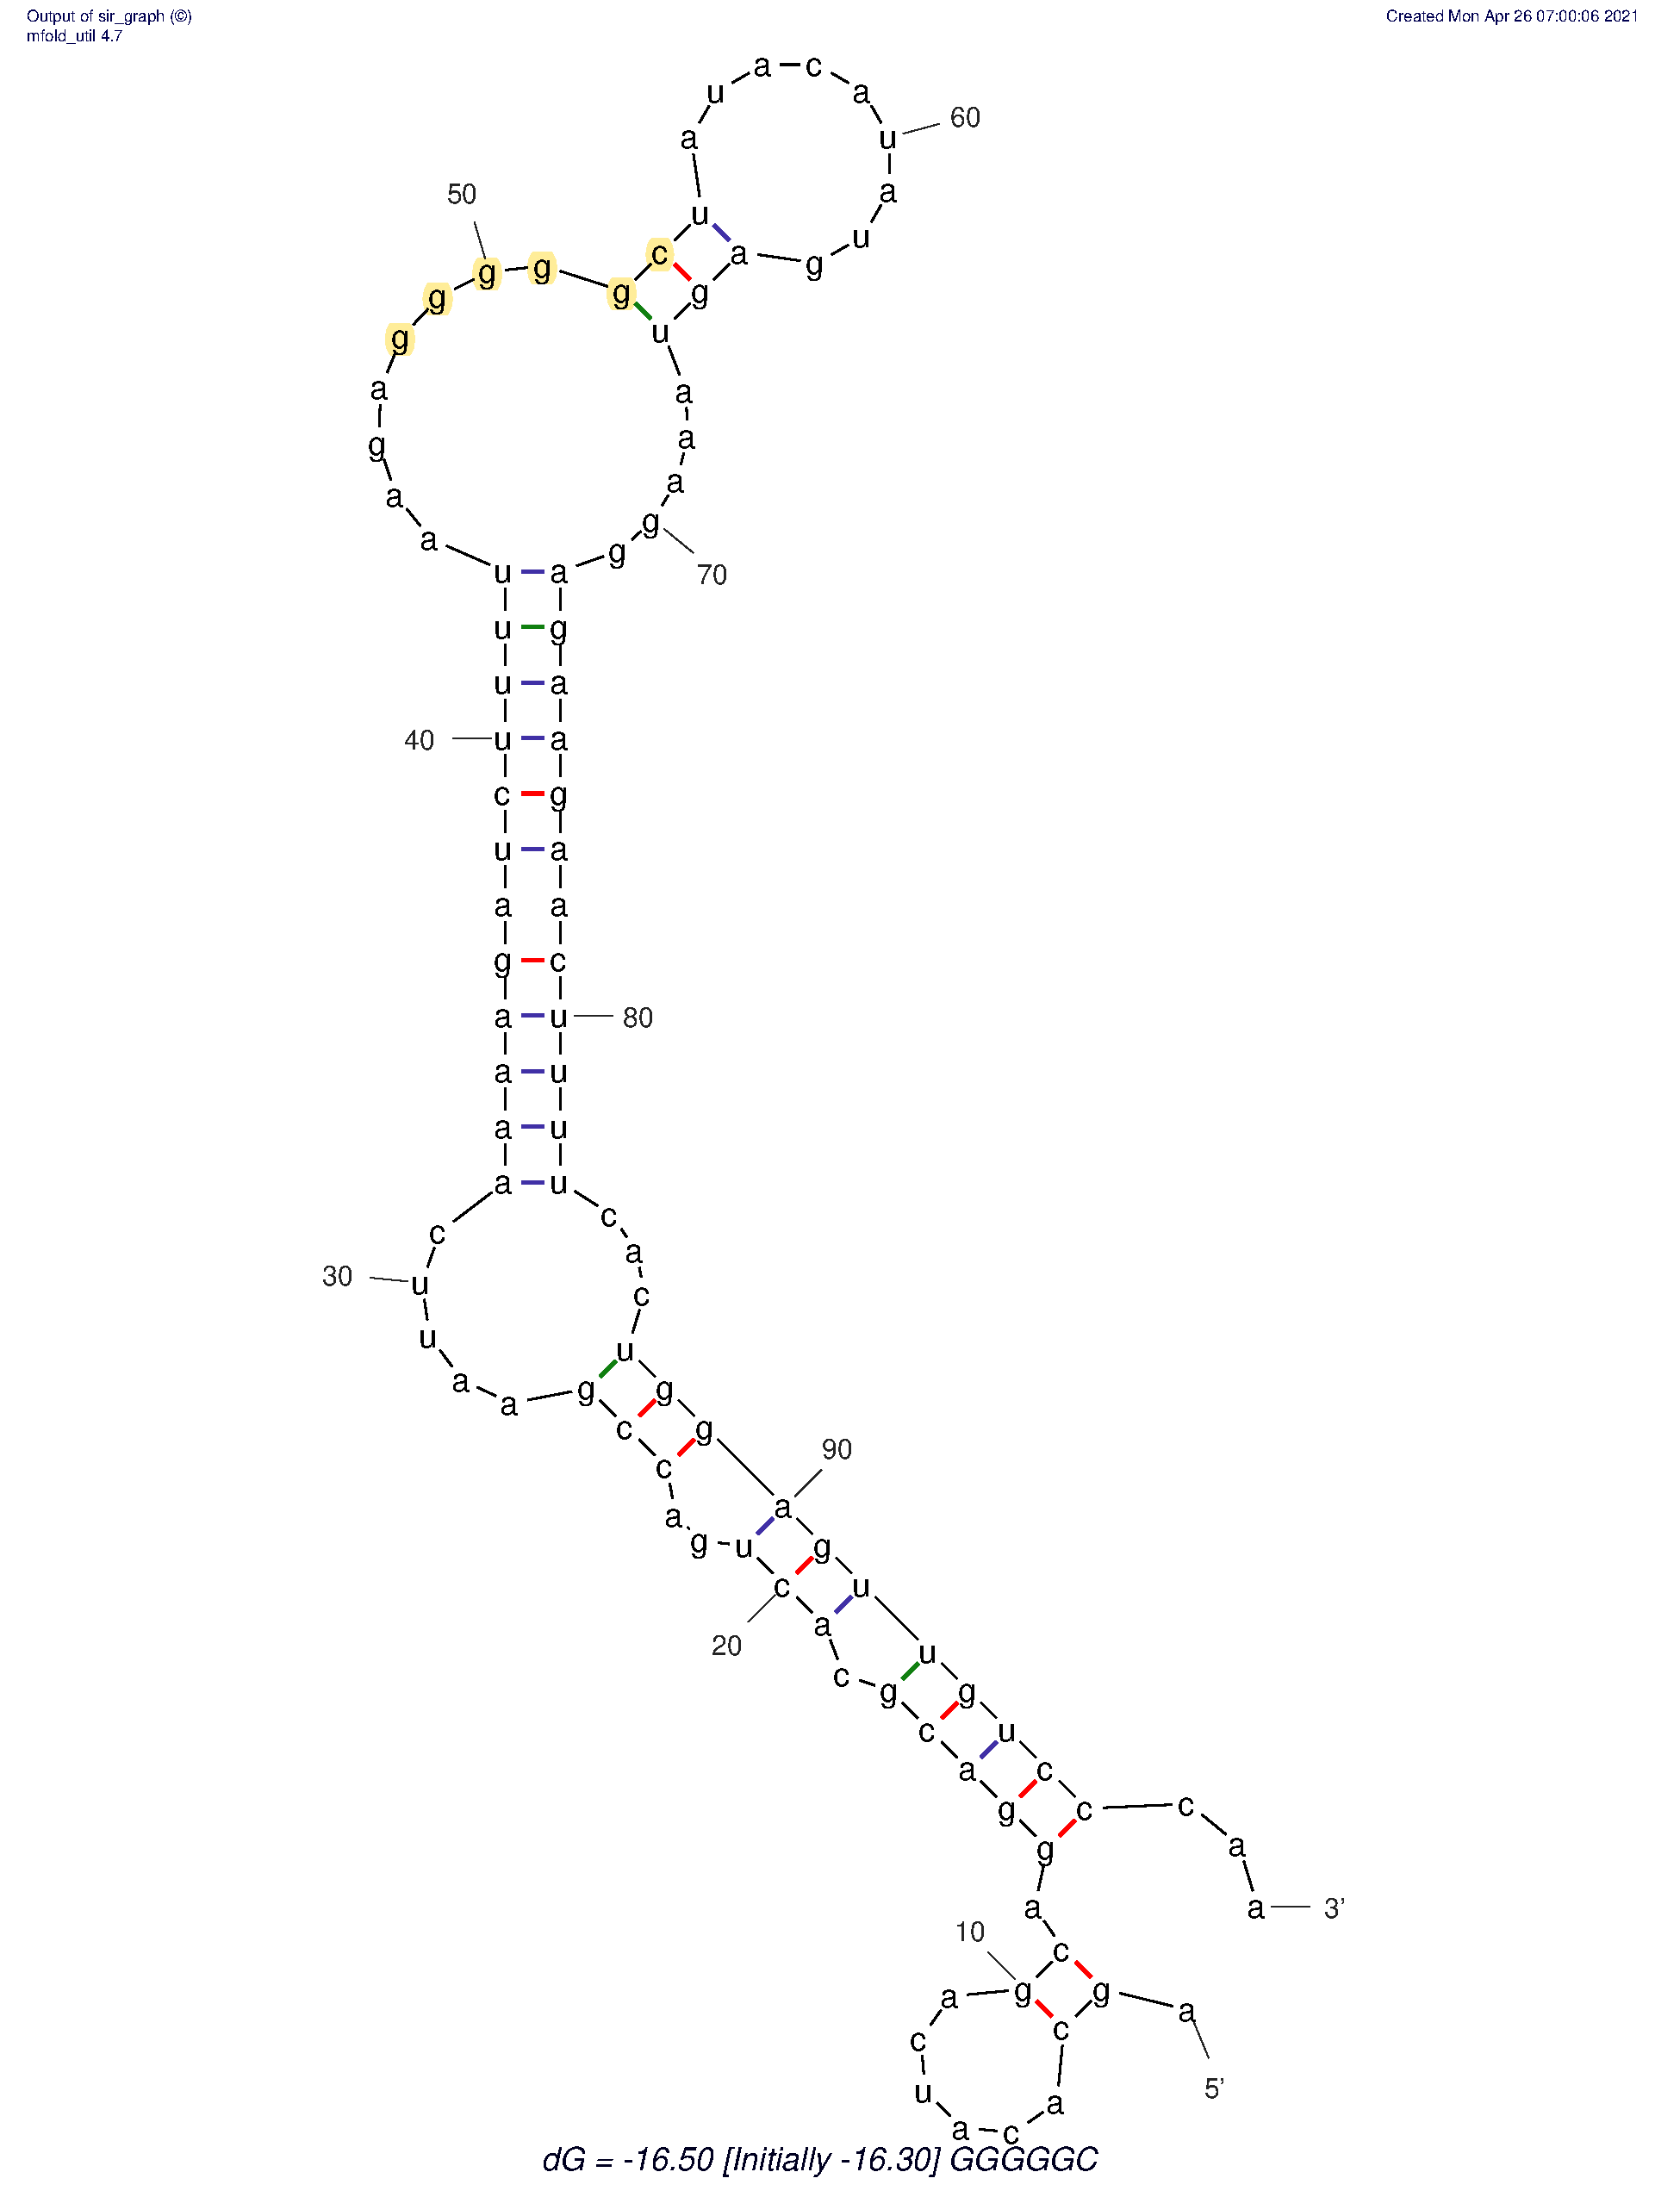
\includegraphics[scale=0.25]{plots/Supplementary/Structure GGGGGC.pdf}
         \caption{$y=3sinx$}
         \label{fig:GGGGGC}
     \end{subfigure}
     \vskip\baselineskip
     \begin{subfigure}[b]{0.49\textwidth}
         \centering
         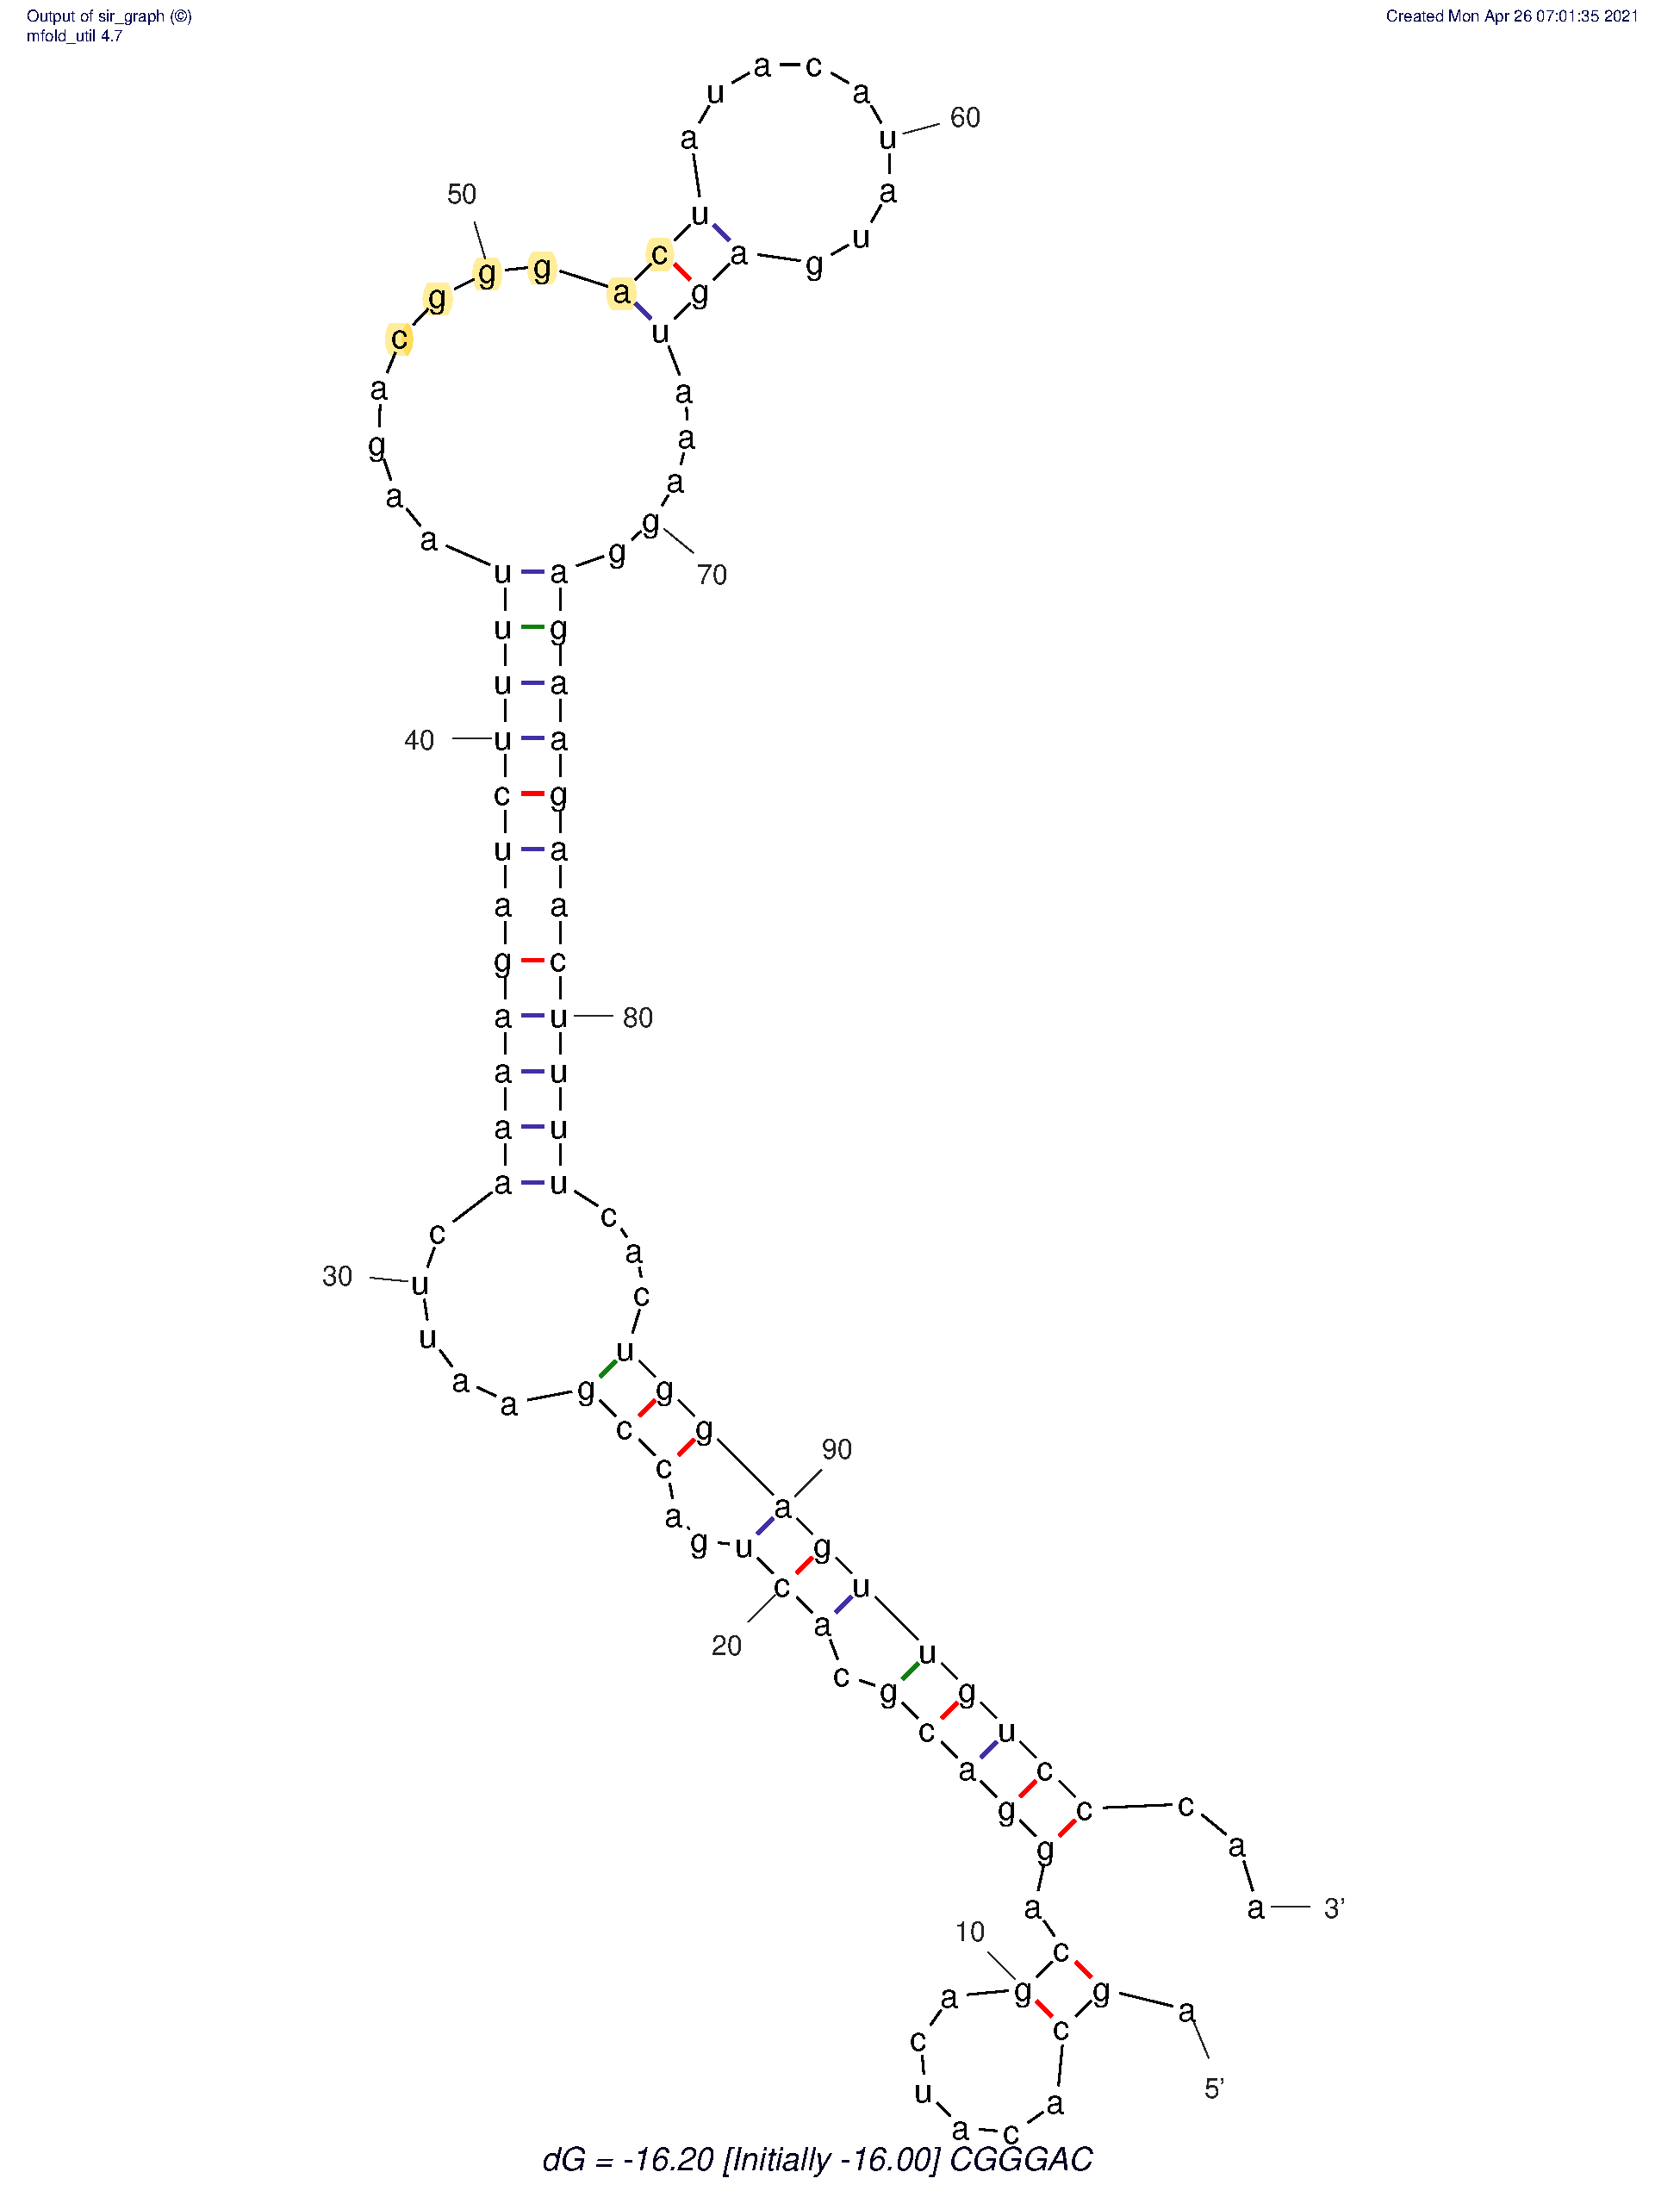
\includegraphics[scale=0.25]{plots/Supplementary/Structure CGGGAC.pdf}
         \caption{$y=5/x$}
         \label{fig:CGGGAC}
     \end{subfigure}
     \hfill
     \begin{subfigure}[b]{0.49\textwidth}
         \centering
         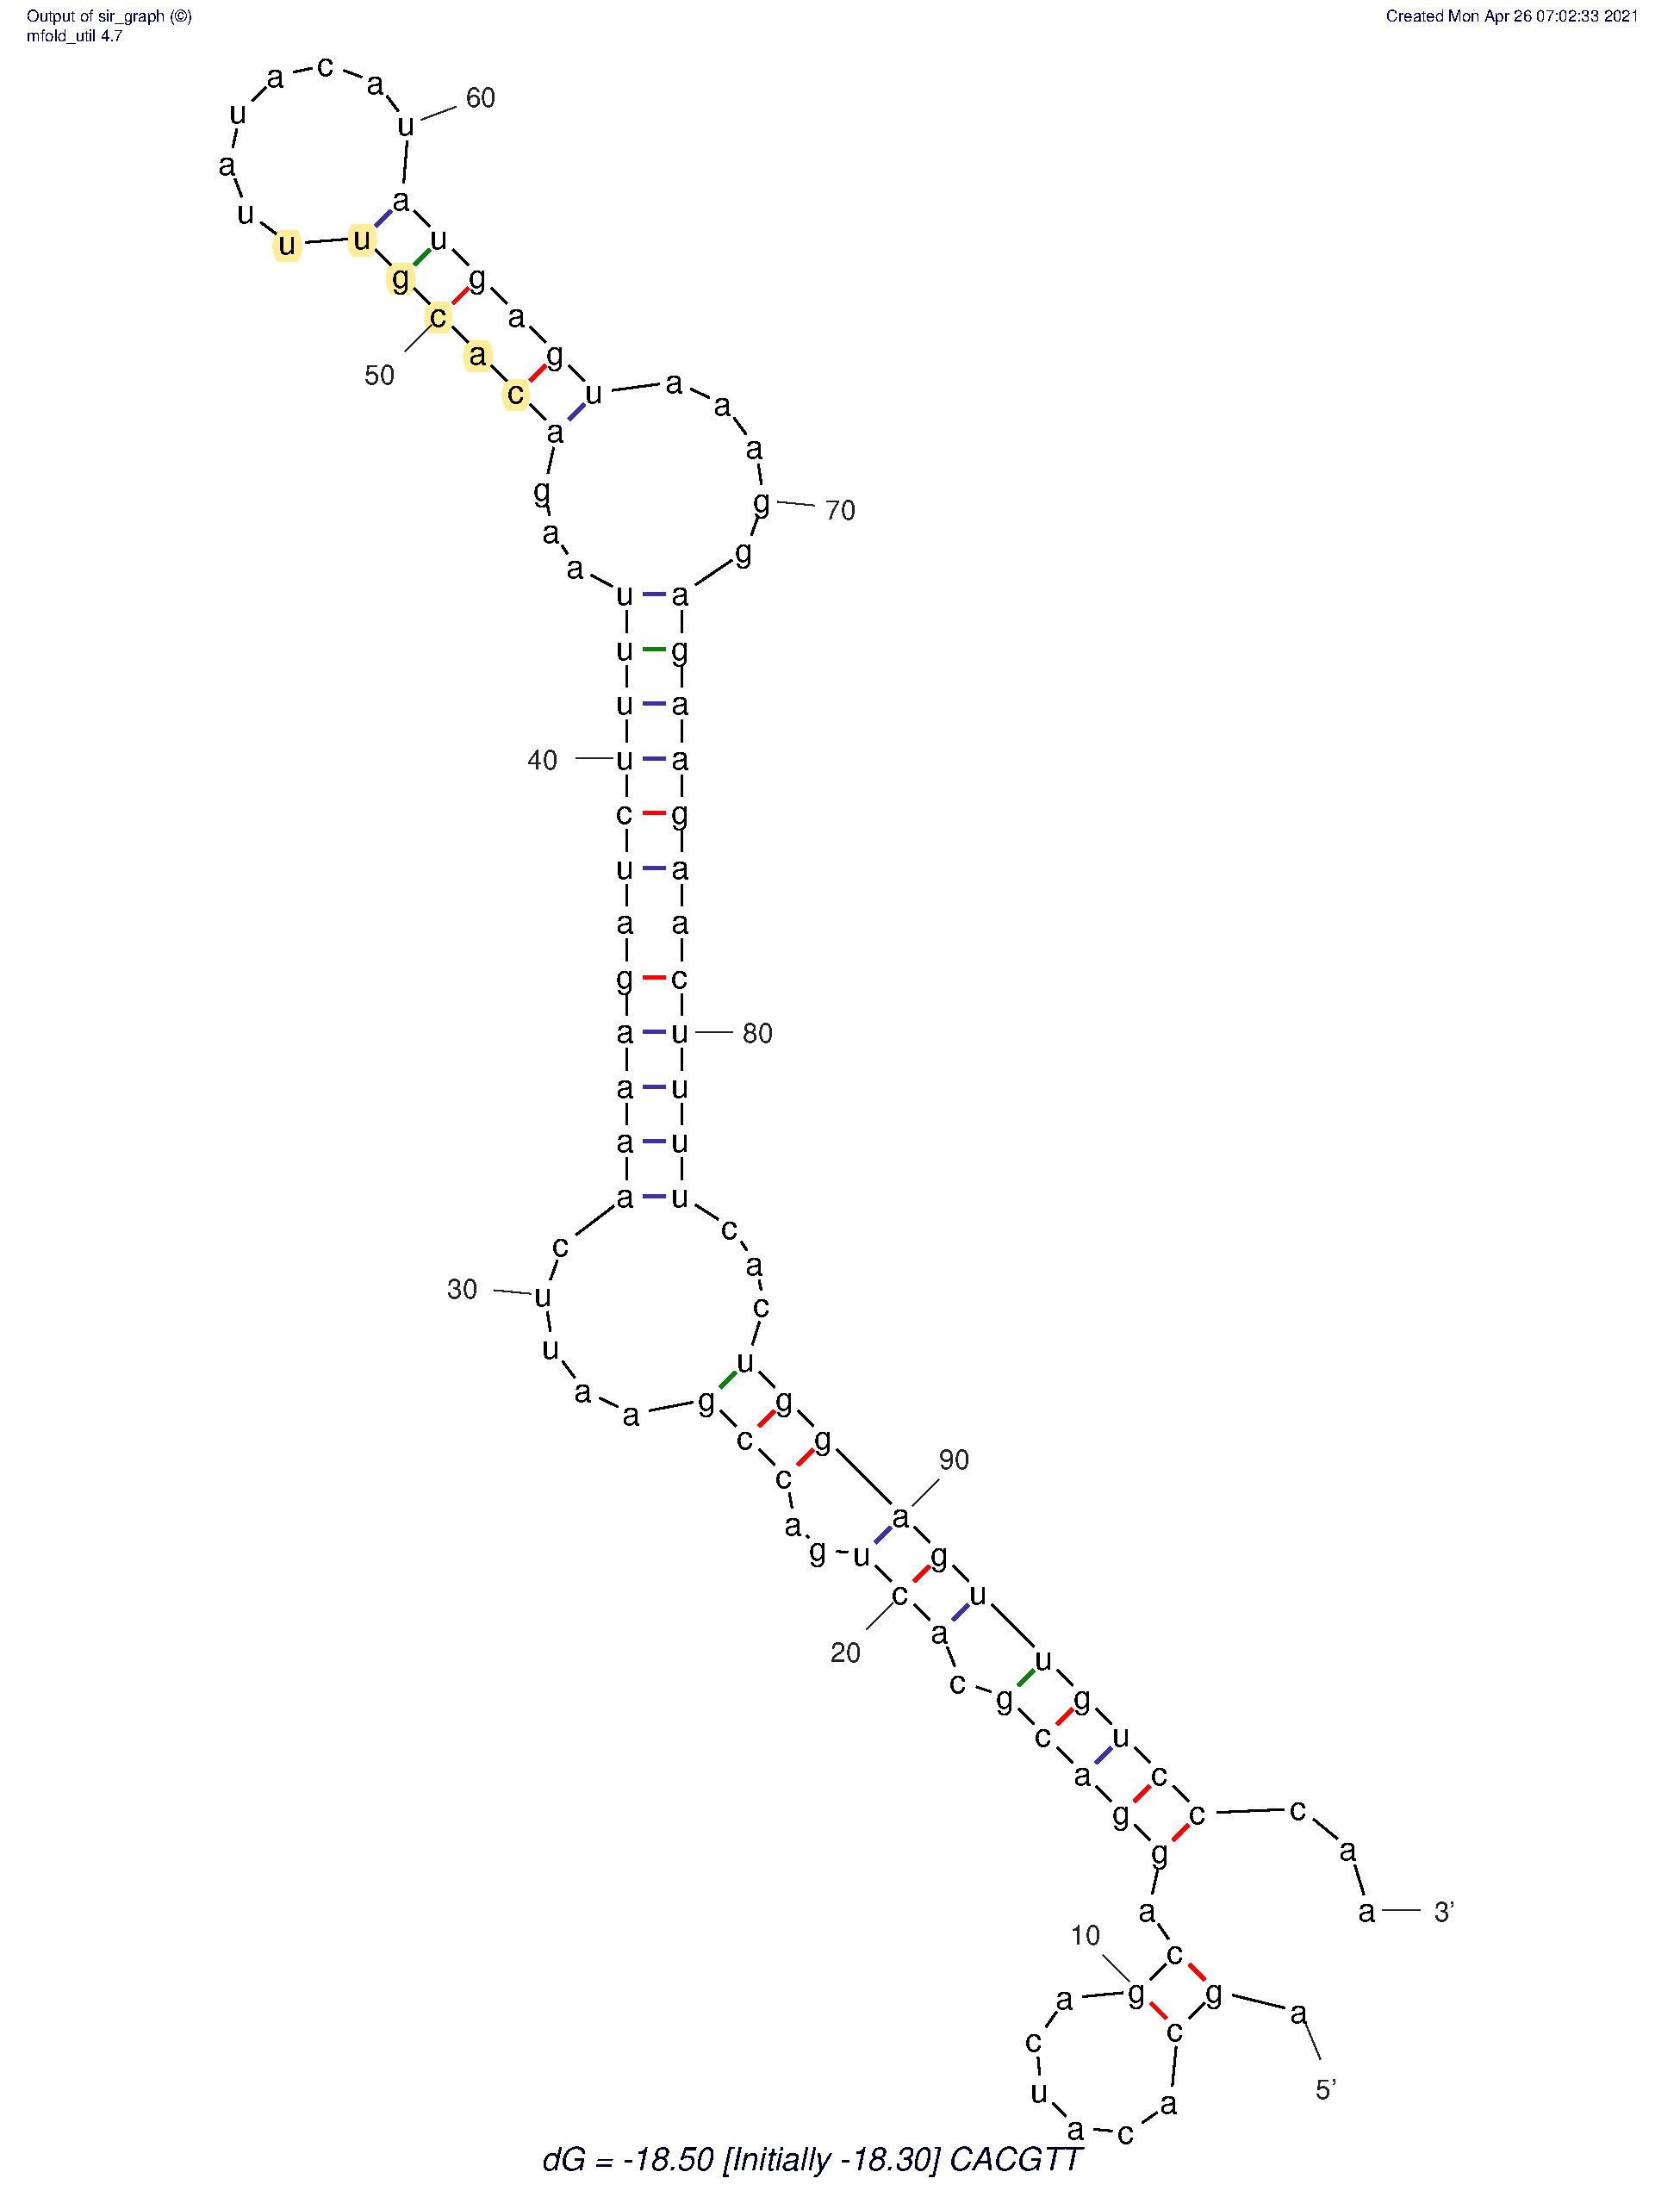
\includegraphics[scale=0.25]{plots/Supplementary/Structure CACGTT.pdf}
         \caption{$y=5/x$}
         \label{fig:CACGTT}
     \end{subfigure}
        \caption{\textbf{Folding predictionds for four different RBS.} Here we show the predicted, energetically most favourable structures for four of our RBS with the following cores: GGGGGG, GGGGGC, CGGGAC, CACGTT and their immediate upstream and downstream background sequence. There is no discerbile and consistent difference between strong ones (the first two) and weak ones (the last two).}
        \label{fig:structures}
\end{figure}


\end{document}
